\documentclass[10pt,spanish,titlepage,letterpaper,openany]{book}
\usepackage[spanish]{babel}
\usepackage[latin1]{inputenc}
\usepackage{titlesec}
\usepackage{enumerate}
\usepackage{anysize}
\usepackage{graphicx}
\usepackage{amsmath}
\usepackage{caption}
\usepackage{subcaption}
\usepackage[nottoc]{tocbibind}
\usepackage{float}
\usepackage{fancyhdr}
\usepackage{color,soul}
\usepackage{amsfonts}
\usepackage{cite}
\usepackage{url}
\usepackage{colortbl}
\usepackage{algorithm}
\usepackage{algorithmic}
\usepackage{multirow} 
\definecolor{black}{rgb}{0,0,0}
\setulcolor{black}

\usepackage{color}
\definecolor{darkgray}{rgb}{0.66, 0.66, 0.66}
\definecolor{editorGray}{rgb}{0.95, 0.95, 0.95}
\definecolor{editorOcher}{rgb}{1, 0.5, 0} % #FF7F00 -> rgb(239, 169, 0)
\definecolor{editorGreen}{rgb}{0, 0.5, 0} % #007C00 -> rgb(0, 124, 0)
\usepackage{upquote}
\usepackage{listings}
\lstdefinelanguage{JavaScript}{
  morekeywords={typeof, new, true, false, catch, function, return, null, catch, switch, var, if, in, while, do, else, case, break},
  morecomment=[s]{/*}{*/},
  morecomment=[l]//,
  morestring=[b]",
  morestring=[b]'
}

\lstdefinelanguage{HTML5}{
        language=html,
        sensitive=true, 
        alsoletter={<>=-},
        otherkeywords={
        % HTML tags
        <html>, <head>, <title>, </title>, <meta, />, </head>, <body>,
        <canvas, \/canvas>, <script>, </script>, </body>, </html>, <!, html>, <style>, </style>, ><
        },  
        ndkeywords={
        % General
        =,
        % HTML attributes
        charset=, id=, width=, height=,
        % CSS properties
        border:, transform:, -moz-transform:, transition-duration:, transition-property:, transition-timing-function:
        },  
        morecomment=[s]{<!--}{-->},
        tag=[s]
}

\lstset{%
    % Basic design
    backgroundcolor=\color{editorGray},
    basicstyle={\small\ttfamily},   
    frame=l,
    % Line numbers
    xleftmargin={0.75cm},
    numbers=left,
    stepnumber=1,
    firstnumber=1,
    numberfirstline=true,
    % Code design   
    keywordstyle=\color{blue}\bfseries,
    commentstyle=\color{darkgray}\ttfamily,
    ndkeywordstyle=\color{editorGreen}\bfseries,
    stringstyle=\color{editorOcher},
    % Code
    language=HTML5,
    alsolanguage=JavaScript,
    alsodigit={.:;},
    tabsize=2,
    showtabs=false,
    showspaces=false,
    showstringspaces=false,
    extendedchars=true,
    breaklines=true,        
    % Support for German umlauts
    literate=%
    {Ö}{{\"O}}1
    {Ä}{{\"A}}1
    {Ü}{{\"U}}1
    {ß}{{\ss}}1
    {ü}{{\"u}}1
    {ä}{{\"a}}1
    {ö}{{\"o}}1
}





\begin{document}
	
	

\renewcommand\thealgorithm{\textcolor{blue}{\thechapter.\arabic{algorithm}}}
\floatname{algorithm}{\textcolor{blue}{Algoritmo}}
\renewcommand{\listalgorithmname}{Lista de algoritmos}
\renewcommand{\algorithmicrequire}{\textbf{Entrada:}}
\renewcommand{\algorithmicensure}{\textbf{Salida:}}
\renewcommand{\algorithmicend}{\textbf{Fin}}
\renewcommand{\algorithmicif}{\textbf{Si}}
\renewcommand{\algorithmicthen}{\textbf{Entonces}}
\renewcommand{\algorithmicelse}{\textbf{Si no}}
\renewcommand{\algorithmicelsif}{\algorithmicelse,\ \algorithmicif}
\renewcommand{\algorithmicendif}{\algorithmicend\ \algorithmicif}
\renewcommand{\algorithmicfor}{\textbf{Para}}
\renewcommand{\algorithmicforall}{\textbf{Para todo}}
\renewcommand{\algorithmicdo}{\textbf{Hacer}}
\renewcommand{\algorithmicendfor}{\algorithmicend\ \algorithmicfor}
\renewcommand{\algorithmicwhile}{\textbf{Mientras}}
\renewcommand{\algorithmicendwhile}{\algorithmicend\ \algorithmicwhile}
\renewcommand{\algorithmicloop}{\textbf{Repetir}}
\renewcommand{\algorithmicendloop}{\algorithmicend\ \algorithmicloop}
\renewcommand{\algorithmicrepeat}{\textbf{Repetir}}
\renewcommand{\algorithmicuntil}{\textbf{Hasta que}}
\renewcommand{\algorithmicprint}{\textbf{Imprimir}} 
\renewcommand{\algorithmicreturn}{\textbf{Retorna}} 
\renewcommand{\algorithmictrue}{\textbf{Cierto }} 
\renewcommand{\algorithmicfalse}{\textbf{Falso }} 
\renewcommand{\algorithmiccomment}[1]{//#1} % mi archivo de traducci�n
\renewcommand{\familydefault}{\sfdefault}%arial
	\begin{titlepage}
		\thispagestyle{empty}
			\begin{figure} [htbp]
				\begin{center}
					
\includegraphics[width=16cm, height = 2cm]{logo}
				\end{center}
			\end{figure}
		%\vspace{1cm}
	%\vspace*{0in}
\begin{center}
\textsl{"LA ESENCIA DE LA GRANDEZA RADICA EN MIS RA�CES"}
\end{center}
\vspace*{1.5cm}


%\begin{Large}
\begin{center}
\textbf{INFORME T�CNICO DE RESIDENCIAS PROFESIONALES}\\
\end{center}
%\end{Large}
\vspace*{1.5cm}


\begin{center}
T�TULO DEL PROYECTO:
\end{center}
\begin{Large}
\begin{center}
\textbf{(AQUI VA EL TITULO DEL PROYECTO)}
\end{center}
\end{Large}
\vspace*{2cm} 


\begin{center}
\textbf{PRESENTA:}\\ (NOMBRE DEL ALUMNO)\\
\bigskip %salto de linea
\bigskip %salto de linea
\textbf{ASESOR:}\\(NOMBRE DEL ASESOR)
\end{center}
\vspace*{2cm}

\begin{figure}[htb]
\begin{flushleft}	

\includegraphics[width=6cm, height=2.5cm]{logo_carrera}
\end{flushleft}
\end{figure}
\vspace*{1cm}

\begin{flushright}
\textbf {Fecha de entrega:} \today
\textbf {.}
\end{flushright}
		\vfill
\end{titlepage}
\setcounter{page}{2}
\begin{center}
\end{center}
	\thispagestyle{empty}
	\newpage

	\newcommand{\bigrule}{\titlerule[0.5mm]}
	\titleformat{\chapter}[display] % cambiamos el formato de los cap�tulos
	{\bfseries\Huge} % por defecto se usar�n caracteres de tama�o \Huge en negrita
	{% contenido de la etiqueta
 	\titlerule % l�nea horizontal
 	\filleft % texto alineado a la derecha
	 	\Large\chaptertitlename\ % "Cap�tulo" o "Ap�ndice" en tama�o \Large en lugar de \Huge
	 	\Large\thechapter} % n�mero de cap�tulo en tama�o \Large
		{0mm} % espacio m�nimo entre etiqueta y cuerpo
	{\filleft} % texto del cuerpo alineado a la derecha
	[\vspace{0.5mm} \bigrule] % despu�s del cuerpo, dejar espacio vertical y trazar l�nea horizontal gruesa
	\pagestyle{fancy}
	\fancyhf{}
	\fancyhead[LO]{\leftmark} % En las p�ginas impares, parte izquierda del encabezado, aparecer� el nombre de cap�tulo
	\fancyhead[RE]{\rightmark} % En las p�ginas pares, parte derecha del encabezado, aparecer� el nombre de secci�n
	\fancyhead[RO,LE]{\thepage} % N�meros de p�gina en las esquinas de los encabezados

	\renewcommand{\chaptermark}[1]{\markboth{\textbf{\thechapter. #1}}{}} % Formato para el cap�tulo: N. Nombre
	\renewcommand{\sectionmark}[1]{\markright{\textbf{\thesection. #1}}} % Formato para la secci�n: N.M. Nombre

	\renewcommand{\headrulewidth}{0.6pt} % Ancho de la l�nea horizontal bajo el encabezado
	\renewcommand{\footrulewidth}{0.6pt} % Ancho de la l�nea horizontal sobre el pie (que en este ejemplo est� vac�o)
	


  % perzonalizar pie de pagina
\renewcommand\thefootnote{\textcolor{blue}{\bf\arabic{footnote}}}

% perzonalizar figuras
  \renewcommand\thefigure{\textcolor{blue}{\thechapter.\arabic{figure}}}
  \renewcommand{\figurename}{\textcolor{blue}{Figura}}
  
  \renewcommand\citeform[1]{\textcolor{blue}{#1}}%cambia el color al texto de las referencias
% perzonalizar tablas

  \renewcommand\thetable{\textcolor{blue}{\thechapter.\arabic{table}}}
  \renewcommand{\tablename}{\textcolor{blue}{Tabla}}
  
% perzonalizar el enumerate
\renewcommand{\labelenumi}{\textbf{\alph{enumi}$)$}} %letras
\renewcommand{\labelenumii}{\textbf{\arabic{enumii}$)$}} %numero arabigos
\renewcommand{\labelenumiii}{\textbf{\Roman{enumiii}.}} %numero ronanos
\renewcommand{\labelenumiv}{\textbf{\fnsymbol{enumiv}}}

\renewcommand{\labelitemi}{$\bullet$}%personaliza los itmes

	\setlength{\headheight}{1.5\headheight} % Aumenta la altura del encabezado en una vez y media

	%\marginsize{3cm}{2cm}{2.5cm}{2.5cm}% Margenes de la pagina

	\renewcommand\listfigurename{Lista de figuras}
	\renewcommand\listtablename{Lista de tablas}
	\renewcommand\listtablename{Lista de tablas}
	\renewcommand\contentsname{Tabla de contenido}
	\renewcommand\bibname{Bibliograf\'ia} %configuracion de tablas y figuras  
 % config de codificacion

\newpage
	%\renewcommand\abstractname{Resumen}
	\pagenumbering{roman}

			%\chapter*{Historia del programa}



	\begin{tabular}{|p{5.5cm}| p{4.5cm}|p{4.5cm}|}\cline{3-3}
		\hline
		\rowcolor[gray]{0.7} Lugar y fecha de elaboraci�n o revisi�n & Participantes & 
		Observaciones (cambios y justificaci�n)\\
		
		Instituto Tecnol�gico de Tl�huac a 3 de Marzo del 2013 & Academia de Sistemas y Computaci�n & Desarrollo del manual\\
		\hline
		Instituto Tecnol�gico de Tl�huac a 30 de Junio del 2014 & Academia de Sistemas y Computaci�n & Modificaci�n y actializaci�n\\
		\hline
	\end{tabular}\\


Nota: Esta secci�n no debe ser incluida en el reporte t�cnico de residencias profesionales.						
			\tableofcontents 
			\listoffigures
			\listoftables
			\listofalgorithms
			\addcontentsline{toc}{chapter}{Lista de algoritmos}  
			\chapter*{Lista de siglas}
	
	\begin{tabbing}
		{\bf\color{white}{Acr�nimo}}    \= {\color{white}{Significado}}\\  
		{\bf{CERN}}   \>  Organizaci�n Europea para la Investigaci�n N�clear, "\textsl{Conseil Europ�en pour la Recherche Nucl�aire}"\\
		{\bf{HTML}}   \>  Lenguaje de Marcas de Hipertexto, "\textsl{HyperText Markup Language}"\\
		{\bf{API}}   \>  Interfaz de Programaci�n de Aplicaciones, "\textsl{Aplication Programming Interface}"\\

		
		

	

				
	
	
	\end{tabbing}
	
			\addcontentsline{toc}{chapter}{Lista de siglas}
			\newpage
		
	\pagenumbering{arabic}	
	
	%\chapter{Introducci�n}

	Una de las partes m�s importantes del trabajo es su introducci�n, ya que es la primera en leerse, y por lo tanto, la que da una idea somera, pero exacta, de los diversos aspectos que componen el trabajo. Se trata, en la �ltima instancia, de hacer un planteamiento claro y ordenado del tema de la investigaci�n, de su importancia e implicaciones, as� como de la manera en la que se ha cre�do conveniente abordar el estudio de sus diferentes elementos. Podr� decirse en consecuencia, que la introducci�n es un anticipo resumido de aquellos temas que despu�s aparecen desarrollados en el trabajo a manera de cap�tulos espec�ficos o secciones tem�ticas. En este sentido, sirve como gu�a y motivaci�n. Bastar� leer la informaci�n en un trabajo serio para decir si interesa o no emprender su lectura a fondo.\\
	
	Una forma efectiva de escribir la introducci�n es tratar de seguir
	el patr�n de un tri�ngulo, esto significa que primero se comienza con afirmaciones generales
	relativas al tema del trabajo reportado en el informe y poco a poco se va precisando m�s
	lo que se dice hasta llegar al meollo del trabajo descrito. Al final de este tri�ngulo se debe
	decir alguna frase o p�rrafo que resuma el contenido del reporte.\\
	
	En t�rminos pr�cticos podr�a decirse que una introducci�n obedece a la formulaci�n de las siguientes preguntas que antes de hacerlas el lector; se ha hecho ya el propio investigado.
	\begin{enumerate}
		\item  �Cu�l es el tema del trabajo?
		\item  �Por qu� se hace el trabajo?
		\item  �C�mo est� pensado el trabajo?
		\item  �Cu�l es el m�todo empleado en el trabajo?
		\item  �Cu�les son las limitaciones del trabajo?
	\end{enumerate}
	Se recomienda que la informaci�n se haga una vez terminado el desarrollo del trabajo, a fin de que no se proponga metas que no se van a alcanzar. En este sentido, no debe confundirse la introducci�n con el plan de trabajo que el investigador elabora al principio, antes de abordar el estudio de los temas propuestos.\\ 
	
	
	El �ltimo p�rrafo de la introducci�n debe contener una descripci�n muy corta, no m�s de una frase, del contenido
	de cada uno de los cap�tulos o secciones en los cuales est� dividido el trabajo. Tal y como se
	hizo en cap�tulo de introducci�n de esta gu�a. La numeraci�n se registra a partir de la introducci�n, 
	siguiendo la numeraci�n subsiguiente.\\
	
	Algunos puntos que el residente debe cubrir en este cap�tulo son:
\begin{enumerate}
	\item Qu� movi� al residente a investigar precisamente este tema o problema y no otro. 

	\item C�mo abord� el tema o el problema (principios, criterios, m�todos y procedimientos).
	
  \item Una descripci�n breve de cada una de las partes del informe desde la justificaci�n hasta las conclusiones y 
				recomendaciones. 	
	
	\item En el caso de que por pol�ticas de la empresa se exija confidencialidad en algunos aspectos del proyecto, esto 
				deber� ser mencionado en la introducci�n.
\end{enumerate}
 
	Dependiendo de la extensi�n del informe completo y de la complejidad, la longitud de
	la introducci�n puede variar, de una p�gina completa como m�nimo a unas cinco o diez
	p�ginas. La introducci�n debe tener sustancia, es decir, su contenido debe transmitir lo
	m�s importante del trabajo reportado en el informe. No debe entrarse en demasiado detalle,
	pero tampoco deben decirse vaguedades, sino aspectos bien concretos del trabajo. Muchas
	personas lo primero que leen son la introducci�n y las conclusiones, para tener una buena
	idea del trabajo realizado, por lo tanto es importante redactar con cuidado
	estas dos secciones, pues son la primera impresi�n que se va a llevar el lector del trabajo.
	En general, la forma como est� escrita esta gu�a debe servir tambi�n de ejemplo de lo
	que es un reporte, c�mo organizarlo y presentarlo.
	

		
	\chapter{Generalidades}
    En este cap\'itulo se presenta de manera detallada los objetivos del proyecto, adem\'as de la informaci\'on de la instituci\'on donde ser\'a desarrollado el mismo.
    
    \section{Objetivos}
    En esta secci\'on se detallan los objetivos tanto generales como espec\'ificos a cumplir a lo largo del desarrollo del Sistema Integral de Indicadores.

\subsection{Objetivo general}

Desarrollar un sistema que permita medir, evaluar y controlar los procesos realizados por cada departamento en el Instituto Tecnol\'ogico de Tl\'ahuac, basado en los lineamientos establecidos por el TecNM en el Sistema de Gesti\'on de Calidad, para lograr realizar una gesti\'on eficaz y de calidad de los mismos.
Este sistema permitir\'a visualizar los resultados de los indicadores de tal manera que los procesos podr\'an ser monitoreados de una manera pr\'actica y accesible.


\subsection{Objetivos espec\'ificos}
\begin{itemize}
    \item An\'alisis de requerimientos.
    \item Toma de datos y entrevistas.
    \item Desarrollo del sistema.
    \item Implementaci\'on de sistema en ambiente de pruebas.
    \item Implemetaci\'on de sistema en ambiende de producci\'on.
\end{itemize}

\section{Justificaci\'on}
\paragraph{}%parrafo 1

Dicho proyecto est\'a basado en la necesidad de contar con una herramienta que permita la evaluaci\'on autom\'atica de los procesos pertenecientes en el Sistema de Gesti\'on de Calidad del Instituto Tecnol\'ogico de Tl\'ahuac, esto debido a que no se cuenta con ning\'un sistema para la realizaci\'on de dicha evaluaci\'on, ya que actualmente los procesos se realizan de manera manual, teniendo as\'i procesos extensos y complicados.
El Sistema Integral de Indicadores facilitar\'a el trabajo realizado, agilizara los tiempos requeridos y permitir\'a con esto brindar un mejor servicio a la comunidad del Instituto Tecnol\'ogico de Tl\'ahuac, adem\'as de que dichos indicadores influyen directamente para la toma de decisiones ya que muestran informaci\'on acerca del cumplimiento de los objetivos, logrando como beneficio el perfeccionamiento de los procesos de la instituci\'on.


\section{Caracterizaci\'on de la empresa en la que particip\'o}
En esta secci\'on se detalla la informaci\'on general de la instituci\'on, as\'i como el \'area para la cual se desarrolla el proyecto.

\subsection{Datos generales de la empresa}
\begin{itemize}
    \item \textbf{Empresa:} Instituto Tecnol\'ogico de Tl\'ahuac.
    \item \textbf{Direcci\'on:} Av. Estanislao Ram\'irez No.301 Colonia Ampliaci\'on Selene C.P. 13420 Tl\'ahuac D.F.
    %\vspace*{1in}
    \begin{figure}[htb]
        \centering
        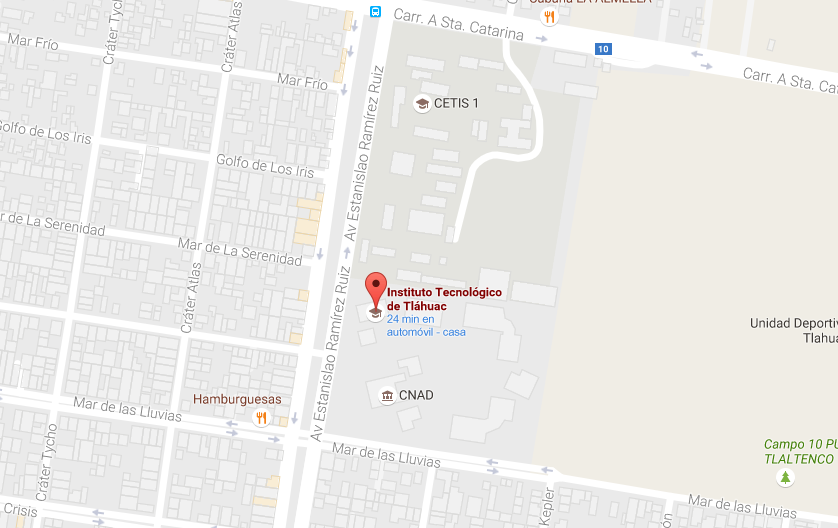
\includegraphics[width=14cm, height=9cm]{figuras/croquis}
        \caption{Croquis de ubicaci\'on.}
        \label{fig_croquis}
    \end{figure}
    \item \textbf{Tel\'efono:} 5866-0927, 7312-5616, 5841-0560, 2594-4096
    \item \textbf{Direcci\'on de correo electr\'onico:} sub.academica@ittlahuac.edu.mx
    \item \textbf{Giro:} Educativo.
    \item \textbf{Misi\'on:} Ofrecer un servicio educativo de calidad a trav\'es de la mejora continua, personal capacitado, compromiso global e infraestructura de vanguardia.

    \item \textbf{Visi\'on:} Ser una instituci\'on de alto desempe\~no acad\'emico, basada en la formaci\'on integral de profesionistas competitivos a nivel internacional con responsabilidad global.

    \item \textbf{Valores:}  Los valores que manejamos en la instituci\'on son los que nos ayudan a identificarnos como seres humanos, como personas que est\'an al servicio de la educaci\'on, que les gusta la actividad que desarrollan y que est\'an orgullosos de promover un servicio de calidad a la comunidad.
    \begin{itemize}
        \item Honestidad.
        \item Respeto.
        \item Trabajo en equipo.
        \item Vocaci\'on de servicio.
        \item Comunicaci\'on.
    \end{itemize}
    \item \textbf{Pol\'iticas de calidad:} La organizaci\'on establece el compromiso de implementar todos sus procesos orient\'andolos hacia la satisfacci\'on de sus estudiantes, sustentada en la calidad del proceso educativo, para cumplir con sus requisitos, mediante la eficacia de un sistema de gesti\'on de calidad de mejora continua, conforme a la norma ISO 9001:2008/NMX-CC-9001-IMNC-2008.
    
    \item \textbf{Estructura organizacional:} La estructura organizacional del Instituto Tecnol\'ogico de Tl\'ahuac se encentra como se muestra en la figura \ref{fig_organigrama}

    \begin{figure}[htb]
        \centering
        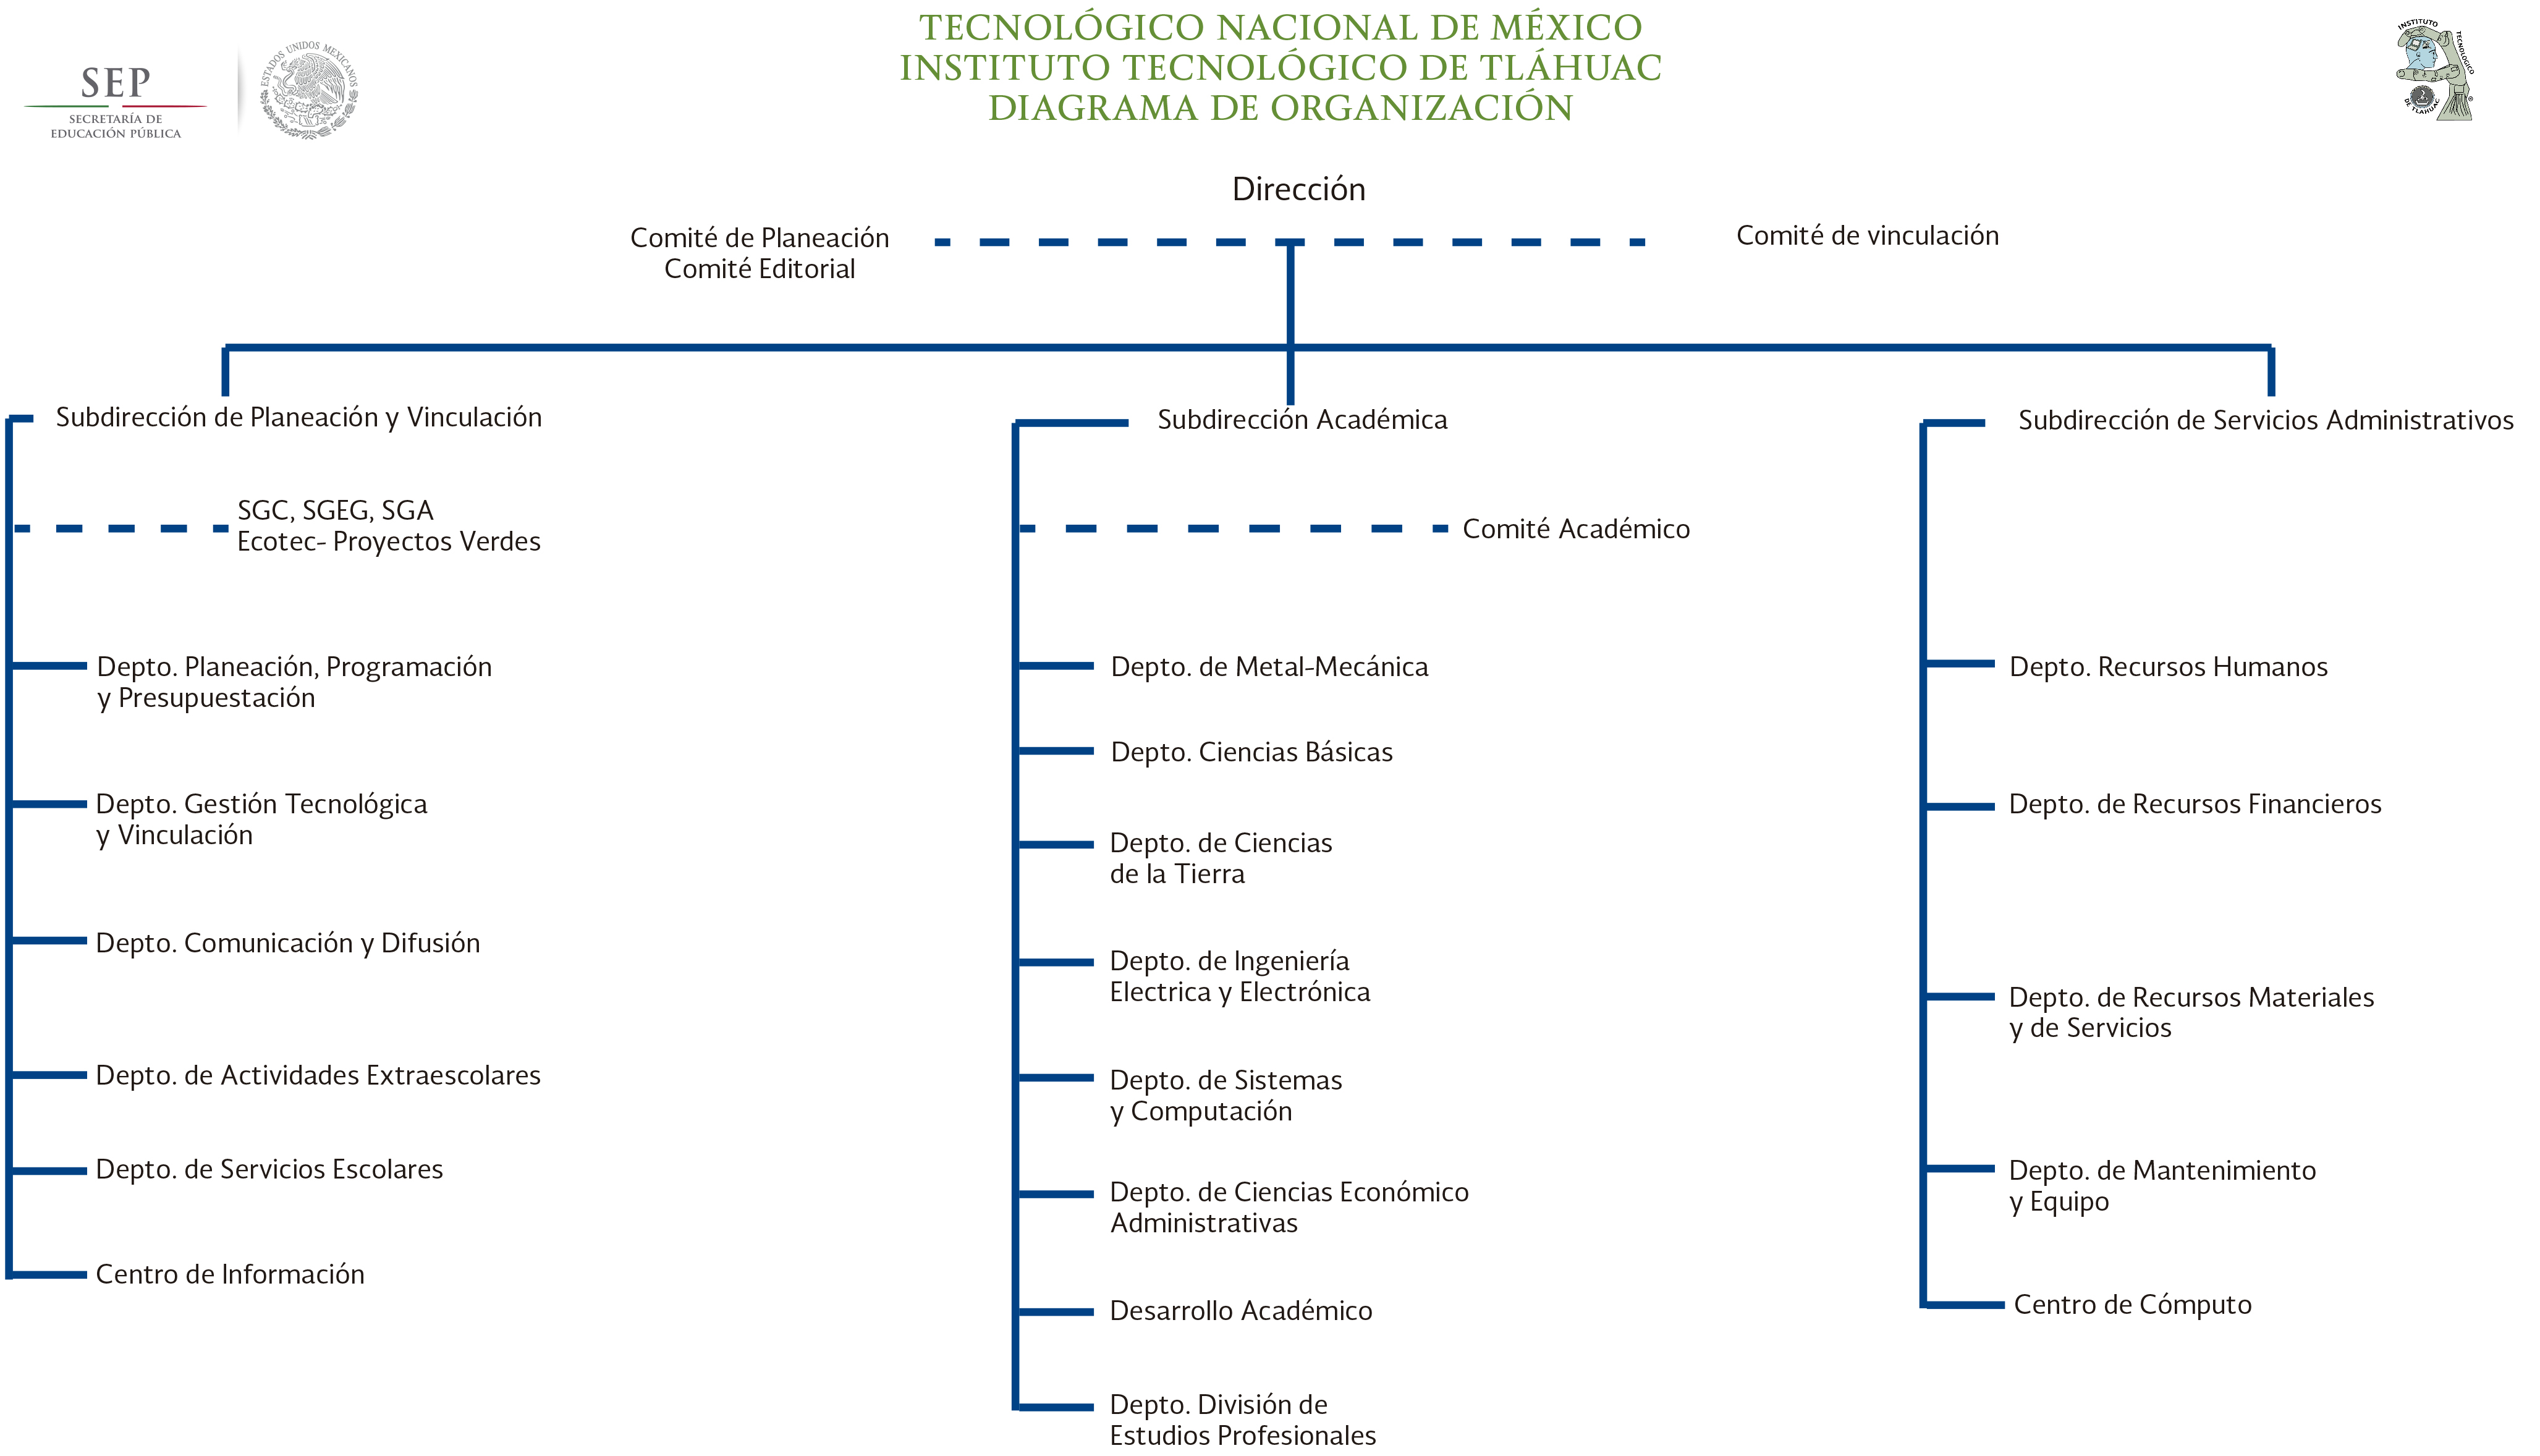
\includegraphics[width=14cm, height=9cm]{figuras/organigrama}
        \caption{Croquis de ubicaci\'on.}
        \label{fig_organigrama}
    \end{figure}
\end{itemize}

\subsection{Descripci\'on del departamento o \'area de trabajo.}
Definicion y detalle de el departamento.

\section{Problemas a resolver}
\paragraph{}%parrafo 1

A continuaci\'on se detallaran los problemas a resolver con el Sistema Integral de Indicadores.

Dentro de los problemas m\'as importantes a resolver se encuentra la digitalizaci\'on de los procesos de indicadores se realizan de manera manual. Esto por ende lleva demasiado tiempo y requiere de una gran sincronizaci\'on entre departamentos para que la informaci\'on sea confiable. Realizar estas actividades requiere de demasiado esfuerzo por parte de los trabajadores del Instituto Tecnol\'ogico de Tl\'ahuac lo que provoca que los tr\'amites sean lentos y tediosos. El Sistema Integral de Indicadores pretende solucionar este problema permitiendo tener la informaci\'on de los procesos en cualquier momento y de una manera sencilla, dando como resultado una sincronizaci\'on de informaci\'on eficiente y por consecuencia procesos m\'as r\'apidos.

Como segundo problema a resolver es la generaci\'on de datos indicadores para la toma de decisiones, la cual de igual manera que los procesos realizados en los departamentos, el sistema permitir\'a configurar reportes de indicadores para los directivos, permitiendo con esto tener informaci\'on general de los procesos.

Como \'ultimo punto el sistema contar\'a con la facilidad de adaptarse a nuevos procesos de indicadores, lo cual permite configurarse de tal manera que cuando la informaci\'on de un indicador cambie, esta modificaci\'on no necesite realizarse un cambio en c\'odigo.

	\chapter{Fundamento te�rico}

	En este cap�tulo se han incluido otros aspectos MUY IMPORTANTES contenidos en
	el reporte, estos aspectos son: la bibliograf�a empleada en el trabajo y las referencias a los
	trabajos de otras personas o de los autores del informe, las cuales se abordan en la secci�n
	4.1; la inclusi�n de figuras y tablas, lo cual se cubre en la secci�n 4.2; consejos muy relevantes
	sobre la edici�n del documento (secci�n 4.3) y las recomendaciones generales sobre redacci�n
	y puntuaci�n que se incluyen en la secci�n 4.4 (material extraido de ~\cite{Ab10}).
	
	\section{La bibliograf�a y las referencias}
	Toda fuente citada en el contenido del informe, debe ser especificada completamente en
	una secci�n denominada bibliograf�a, referencias bibliogr�ficas o simplemente referencias. La
	bibliograf�a generalmente se refiere s�lo a libros utilizados en el trabajo, sin embargo las
	referencias s� pueden incluir art�culos de revistas, sitios web, libros y otros y se especifican
	completamente, incluyendo n�mero de p�ginas, fecha de publicaci�n, autores, t�tulo completo, 
	y los detalles de d�nde apareci�. Si se trata de un art�culo en una revista (publicaci�n
	peri�dica), se deben colocar, adem�s de los datos del art�culo en cuesti�n, el t�tulo de la revista,
	el volumen, el n�mero y el a�o. Es esencial utilizar una notaci�n est�ndar para enumerar
	las referencias, hay varios estilos usados en la literatura actual. Uno de estos estilos es listar
	las referencias en orden de cita dentro del texto y numerarlas del [1] hasta el �ltimo n�mero
	necesario para numerarlas todas. Otro estilo es ordenarlas por el apellido del primer autor y
	la manera abreviada de hacer referencia a cada una de ellas es con las 3 � 4 primeras letras
	del apellido del primer autor, o con las iniciales del primer apellido de todos los autores y
	al final de estas letras los dos �ltimos d�gitos del a�o de publicaci�n de la referencia. Por
	ejemplo, si se va a citar el art�culo ''Lineamientos sobre c�mo escribir informes t�cnicos'' de Soraya
	Abad-Mota, se puede hacer referencia a �ste como: ~\cite{Ab10}. En
	ingl�s es com�n encontrar la palabra ''references'' para la secci�n que contenga las referencias, 
	sin embargo en castellano es m�s com�n utilizar la palabra ''bibliograf�a'' para ello, a�n
	cuando �sta incluya referencias a fuentes que no son libros, como se hace en esta gu�a, por
	ejemplo.\\
	
	Todas las fuentes que aparecen en la bibliograf�a deben ser citadas en alguna parte del
	texto, por otro lado, todas las fuentes citadas en el texto deben aparecer completas en la
	secci�n o cap�tulo de Bibliograf�a. Cuando se cita una fuente, basta con hacer referencia a la
	numeraci�n utilizada en la bibliograf�a, no se debe copiar dos veces la referencia completa,
	para eso est� la secci�n de bibliograf�a, para colocar la cita completa. Adem�s de colocar la
	numeraci�n de la cita, uno puede hacer referencia al autor o autores de la misma, como se
	hace en la siguiente frase: ''Matthieu Crussi\`ere en ~\cite{Cr05} trata el tema del env�o de datos
	por la red el�ctrica''. En las cita se puede hacer referencia a una fuente de varios autores, 
	se puede dar el nombre del primer autor y las palabras ''et al.'', las cuales constituyen una 
	abreviatura de ''et alia'' que significa ''los otros'' en lat�n.\\
	
	Es importante recordar que el reporte lo redacta el autor del mismo utilizando sus propias
	palabras, si es necesario colocar citas textuales de trozos redactados por otros autores es
	obligatorio colocar esos trozos entre comillas ('' '') y citar la fuente donde apareci� el trozo.
	Nunca se debe colocar sin comillas, ni dar la impresi�n de que uno escribi� algo que en
	realidad no ha escrito. Por ejemplo, cuando en una residencia, se va a describir a la
	empresa es t�pico usar alg�n folleto o p�gina web de la empresa, si se van a usar trozos
	de esa descripci�n en el reporte, se deben colocar entre comillas y citar la fuente, la cita
	completa del folleto o la p�gina web debe aparecer en la bibliograf�a.\\
	
	Finalmente, como ejemplos de varios tipos de fuentes se incluyen en la Bibliograf�a las
	siguientes referencias: ~\cite{ChJo99} y ~\cite{ElNa99}.
	
	
	\begin{figure}[b]
	\centering
		
\includegraphics[width=.2\textwidth, height = .2\textwidth]{./figuras/Fig1}
	\caption{Pie de figura.}
	\label{fig:Fig1}
\end{figure}
	
	\section{Inclusi�n de figuras y tablas}
	Algunos informes requieren la inclusi�n de figuras o de tablas, las cuales deben estar
	numeradas seg�n el cap�tulo en el cual aparece. Puede utilizarse una numeraci�n separada para cada cosa, 
	es decir una numeraci�n para las figuras y otra aparte para las tablas. Al pie de cada figura o 
	cabecera de cada tabla debe aparecer una nota que diga ''\textcolor{blue}{Figura} ~\ref{fig:Fig1}: t�tulo de la figura'' o 
	''\textcolor{blue}{Tabla} ~\ref{tab:expre}: T�tulo de la tabla'', respectivamente. Tanto las figuras como las tablas deben 
	anunciarse y explicarse en el texto y deben ir ubicadas cerca del texto que las describe.
	Generalmente, despu�s de la tabla de contenido de todo el informe, se colocan el �ndice
	de figuras, donde para cada figura se coloca su t�tulo y la p�gina donde aparece, 
	y el �ndice de tablas, donde para cada tabla se indican su t�tulo y la p�gina donde aparece.\\
	
	Como nota final, es �til anunciar que si se va a elaborar un informe largo donde se tomen
	en cuenta todos los aspectos de presentaci�n descritos en esta gu�a, pueden revisar el paquete
	LaTex de formateo de texto, que es muy poderoso y con el cual se han publicado muchos
	libros. Esta gu�a fue realizada en LaTex.
	
	

\begin{table}[t]
				\begin{center}
				  \caption{Notaci�n del sistema de prueba.}
				  \scalebox{0.8}{
					\begin{tabular}{ l l c c}
					\hline
					Expresi�n & Comentario & Longitud (muestras) & M�dulo\\
					\hline
  
					$\vec{\mathbf{v}}_{on-off}$     & Secuencia binaria    & $b*M$ & Informaci�n fuente\\
					$\vec{\mathbf{v}}_{piloto}$     & Secuencia binaria constante  & $64$ & Informaci�n fuente\\
					$\vec{\mathbf{v}}_{on-off-A}$   & Secuencia binaria del s�mbolo piloto tipo ''A''    & $b*M$ & Informaci�n fuente\\
					$\vec{\mathbf{v}}_{on-off-R}$   & Secuencia binaria del s�mbolo tipo ''R''    & $b*M$ & Transmisor\\
					$\vec{\mathbf{v}}_{antipodal}$  & Secuencia antipodal  & $b*M$ & Transmisor\\
					\hline
					\end{tabular}}
					\label{tab:expre}
				\end{center}
			\end{table}
	
\section{Ecuaciones}

Por favor utilice s�mbolos que est�n disponibles en  ingl�s y en espa�ol, en las versiones de procesadores de textos. Las ecuaciones deber�n estar numeradas con el n�mero entre par�ntesis y al margen derecho del texto, Ej.

 		          \begin{equation}
               Y = 4x^{2} - 3x + 5  \label{ecua}
          \end{equation}
          
Para su menci�n utilice:  ecuaci�n ~\ref{ecua}. 	
	
\section{Edici�n del documento}
	
Esta gu�a incluye las descripciones completas de los tipos de letra, del espaciamiento y la informaci�n relacionada para elaborar sus reportes, basada en los formatos utilizados por la IEEE.

\subsection{Caracter�sticas generales}

Todo el material impreso, incluyendo el texto, las ilustraciones, y los gr�ficos, se deben mantener dentro de un �rea de impresi�n de 17,5 cm ancho por 23 cm alto. No escriba, ni imprima nada fuera del �rea de impresi�n. Todo texto debe estar en un formato de una columna. El texto debe estar justificado.\\

Este documento es un  ejemplo del formato con los m�rgenes y la colocaci�n del texto, �ste est� disponible en formato de WORD y PDF. Contiene las l�neas y los p�rrafos con los m�rgenes y �rea de impresi�n. Las caracter�sticas generales del texto deben de respetar los siguientes criterios:

\begin{itemize}
	\item Los escritos deben ser impresos en hojas tama�o carta, (21.5 cm x 27.9 cm).
	\item En las p�ginas impares, parte izquierda del encabezado, aparecer� el nombre de cap�tulo.
	\item En las p�ginas pares, parte derecha del encabezado, aparecer�a el nombre de secci�n.
	\item Los m�rgenes externos deben de respetar los siguientes criterios:
		\begin{itemize}
			\item Margen izquierdo: 2.0 cm para p�ginas pares y 3.5 p�ginas impares.
			\item Margen derecho: 3.0 cm para p�ginas pares y 2.0 p�ginas impares.
			\item Margen superior: 2cm.
			\item Margen inferior: 2cm.
		\end{itemize}
\end{itemize}

\subsection{T�tulo principal de cap�tulo}

El t�tulo principal debe tener una alineaci�n a la derecha, junto con el n�mero y nombre del cap�tulo. El n�mero debe ser escrito en n�mero romano. Esta gu�a presenta el ejemplo adecuado para los t�tulos de cada cap�tulo.


\subsection{Tipos de letra}

Cualquier tipo de letra Arial es aceptada, Arial Narrow o Arial Unicode MS pueden ser utilizadas. Es permitido utilizar tipo de letra Times New Roman en lugar de tipo Arial, pero debe utilizarse el mismo tipo de letra en todo el documento y aumentar en 1 punto el tama�o respecto de los que se se�alan en el presente documento.\\ 
Nota: Por favor evite hacer uso de tipos de letra del mapa de caracteres que no sean los autorizados.

\subsection{Texto principal}

Escriba su texto en Arial de 10 pts, espacio simple. No utilice el doble espaciamiento. Todos los p�rrafos deber�n iniciar con una sangr�a de 0.75 cm en el primer rengl�n y justificados. Por favor deje un espacio en blanco entre p�rrafos.\\ 

Los t�tulos de la figura y de las tablas deben ser en Arial de 9 pts. Use may�sculas s�lo en la primer palabra de cada t�tulo de las figuras y de las Tablas. Las figuras y las tablas se deben numerar separadamente. Los t�tulos de la figura deber�n estar centrados debajo de las figuras. Los t�tulos de las tablas deber�n estar centrados arriba de las tablas. 



\section{T�tulo de primer nivel (secci�n)}

Por ejemplo, ''4.4. T�tulo de primer nivel'', en Arial, negrita de 12 pts,  justificado, con un espacio en blanco antes y un espacio en blanco despu�s.

\subsection{T�tulo de segundo nivel (subsecci�n)}

Cuando sea necesario este t�tulo, deben ser en Arial, negrita, de 11 pts, justificado, con un espacio en blanco antes, y un espacio en blanco despu�s. Por ejemplo: ''4.3.1. Caracter�sticas generales''

\subsubsection{T�tulo de tercer nivel}

Los t�tulos de tercer orden no son recomendables pero si es necesario, deben ser en Arial de 10 pts, en negritas, justificado con un espacio en blanco antes, y un espacio en blanco despu�s. Este nivel no lleva numeraci�n, tal y como se aprecia  en este ejemplo (T�tulo de tercer nivel).


		
			




	
	\chapter{Desarollo}

	Dentro de este cap\'itulo se desglosar\'an las etapas que se siguieron en el desarrollo del SII, cada una de estas es parte de la metodolog\'ia de cascada que fue la que se eligi\'o para este desarrollo.

	\section{An\'alisis del sistema}
		Una de las actividades m\'as importantes del Instituto Tecnol\'ogico de Tl\'ahuac es el c\'alculo de indicadores, esto debido a que estos brindan informaci\'on para la mejora de los procesos. El Sistema Integral de Indicadores debe ser capaz de mostrar la informaci\'on requerida por los usuarios de una manera f\'acil, flexible y r\'apida.\\

		La informaci\'on que se requiere del sistema es el seguimiento de los procesos de los diferentes departamentos. Los departamentos a administrar por el sistema son los siguientes:

		\begin{itemize}
			\item Acad\'emico.
			\item Vinculaci\'on.
			\item Planeaci\'on.
			\item Administraci\'on de los recursos.
			\item Calidad.
		\end{itemize}

		Cada uno de ellos requiere obtener informaci\'on espec\'ifica la cual permitir\'a mejorar cada uno de sus procesos.

		El sistema ser\'a capaz de recalcular los indicadores con los cambios que se le presenten a lo largo del periodo declarado, permitiendo con esto tomar decisiones estrat\'egicas para mejorar en caso de que los indicadores sean bajos, o mantener las buenas pr\'acticas en caso de que los indicadores sean los esperados.\\

		Los reportes a configurar dentro del sistema contendr\'an un n\'umero indefinido de c\'alculos, es decir, el n\'umero de datos a calcular es din\'amico permitiendo con esto darle flexibilidad y adaptaci\'on a diferentes circunstancias.\\


		Se necesita que el sistema tenga las siguientes caracter\'isticas:

		\begin{itemize}
			\item \textbf{Configurable:} El sistema debe tener la capacidad de ser configurado de acuerdo a las necesidades de los usuarios.
			\item \textbf{Escalable:} El sistema debe de ser capaz de adaptarse a nuevas funcionalidades y nuevos m\'odulos, esto quiere decir que debe estar listo para que nuevos desarrolladores puedan usar como base este desarrollo para futuras adaptaciones.
			\item \textbf{Amigable:} Es importante que la presentaci\'on del sistema sea agradable para el usuario, debido a que esto mejora la experiencia del mismo permitiendo al usuario tener un ambiente de trabajo agradable.
		\end{itemize}
		
		Con estas tres caracter\'isticas el sistema debe ser capaz de calcular y mostrar las cifras de los indicadores por departamento.

	\section{An\'alisis de requisitos del software}

		Para la realizaci\'on del Sistema Integral de Indicadores se requiere que este se desarrolle en un ambiente Web, esto para permitir que multiples usuarios puedan acceder a estos datos simult\'aneamente.\\

		A lo largo de esta secci\'on se detallaran los distintos tipos de requerimientos necesarios para el desarrollo del sistema.\\

		\subsection{Requerimientos f\'isicos}
			Para el correcto funcionamiento del sistema es necesario contar con el equipo y software  adecuado, del cual hablaremos a continuaci\'on:

			\begin{itemize}
				\item Hardware
					\begin{itemize}
						\item \textbf{Servidor 1:} Equipo con Windows Server 2012 R2 (recomendado) o alg\'un sistema operativo con Windows a 64 bits dedicado para el servidor de base de datos. M\'inimo 4GB de RAM, para su correcto funcionamiento se necesitan 6 GB o m\'as, Procesador x64 a 1.4 GHz, para su correcto funcionamiento procesadores a 2.0 GHz o m\'as. M\'inimo 6GB de disco duro para su instalaci\'on, el tama\~no del disco duro depende a las demandas de espacio al ir almacenando informaci\'on.

						\item \textbf{Servidor 2:} Equipo con Windows Server 2012 R2 (recomendado) o alg\'un sistema operativo con Windows a 64 bits dedicado para el servidor de aplicaci\'on. M\'inimo 2GB de RAM, para su correcto funcionamiento se necesitan 4 GB o m\'as, Procesador x64 a 1.4 GHz, para su correcto funcionamiento procesadores a 2.0 GHz o más. Disco duro de 500GB para almacenamiento de sitios y archivos en servidor.

						\item \textbf{Desarrollo:} Equipo con Windows Server 7 Ultimate a 64 bits dedicado para el desarrollo del sistema, 6GB de RAM o m\'as. Procesador x64 a 1.4 GHz, para su correcto funcionamiento procesadores a 2.0 GHz o m\'as. Disco duro de 500GB para almacenamiento de fuentes y archivos de instalaci\'on.

					\end{itemize}
				\item Software
					\begin{itemize}
						\item Microsoft SQL Server 2012.
						\item IIS Server 8.0 o superior.
						\item Navegador Web (Mozilla Firefox preferentemente)
						\item Microsoft Visual Studio 2013 Test Premium
					\end{itemize}
			\end{itemize}

		El servidor 1 deber\'a tener instalado Microsoft SQL Server 2012 para fungir como servidor de base de datos.\\

		El servidor 1 deber\'a tener instalado IIS Server 8.0 para fungir como servidor de aplicaci\'on y almacenamiento de archivos.\\

		El equipo de desarrollo deber\'a tener instalado Microsoft Visual Studio 2013 Test Premium, Navegador Web adem\'as de IIS Server 8.0 para fungir como ambiente de desarrollo.\\

		\subsection{Interfaces}
		
			El Sistema Integral de Indicadores ser\'a un sistema alimentado de todas las tablas del sistema general. Para esto es necesario establecer los m\'etodos de entrada y salida de datos.\\

			\subsubsection{Entrada de datos}

				Para la entrada de datos es necesario contar con una serie de configuraciones que permitan obtener la informaci\'on de cualquier tabla de la base de datos, esto permitir\'a obtener datos din\'amicos adaptables a las necesidades que tenga en ese momento el usuario.

				Los m\'odulos para realizar la configuraci\'on del sistema son:
				\begin{itemize}
					\item \textbf{Departamentos:} En este m\'odulo se permitir\'a declarar la informaci\'on de los departamentos que se manejar\'an en el SII, los datos requeridos hasta el momento son Id, nombre y descripci\'on.
					\item \textbf{Formulas:} En este m\'odulo se configurar\'an las f\'ormulas que extraer\'an los datos de la base de datos y realizaran los c\'alculos establecidos en estas. Los campos requeridos para configurar una formula son id formula, nombre y la definici\'on de la formula.
					\item \textbf{Colecciones:} Este m\'odulo permite establecer las f\'ormulas que se aplicaran a cada proceso. Las formulas pueden estar en m\'as de un proceso, esto debido a que se puede reutilizar un cálculo de un departamento a otro. Los campos necesarios en este m\'odulo solamente son el id de formula y el id de colecci\'on.
					\item \textbf{Procesos:} En este se definen los datos del periodo dentro de los cuales se necesitan el departamento al que pertenece, numero interno de proceso, descripci\'on, grupo de f\'ormulas a aplicar, fecha de inicio y fin, responsable y unidad de medida.
				\end{itemize}

			\subsubsection{Salida de datos}

				Para la salida de datos se necesita hasta el momento una sola vista en donde se ve el resultado del proceso del periodo de indicadores, esta secci\'on mostrara los siguientes datos:
				\begin{itemize}
					\item \textbf{N\'umero interno de periodo de indicadores:} El n\'umero interno del periodo de indicadores es el identificador \'unico para cada periodo de indicadores.
					\item \textbf{N\'umero consecutivo:} Este se asignar\'a al momento de resolver la formula d\'andole a cada registro del detalle del proceso un identificador.
					\item \textbf{Formula sistema:} Aqu\'i se mostrar\'a la formula tal cual est\'a en el sistema al momento del proceso.
					\item \textbf{Formula pre compilado:} En esta se resuelven las funciones propias del sistema, es decir, las formulas programadas en el sistema, dando como resultado una formula la cual se encuentra lista para ser resuelta por el m\'odulo de f\'ormulas de Microsoft Excel.
					\item \textbf{Resultado:} En este se mostrara el resultado de la formula resuelta por Excel y ser\'a el dato m\'as interesante ya que ser\'a el resultado del indicador.
					De los datos insertados en el sistema, el que requiere de especial atenci\'on es la definici\'on de la formula, esto debido a que si existe alg\'un error en sintaxis al momento de procesar la formulas, esta retornara un valor de 0.
				\end{itemize}

		\subsection{Usuarios y factores humanos}

			El Sistema Integral de Indicadores est\'a pensado para tres tipos de usuarios de usuarios los cuales tendr\'an roles y permisos diferentes. Los usuarios que se podr\'an usar en el sistema son los siguientes:

			\begin{itemize}
				\item Usuario administrador.
				\item Usuario soporte
				\item Usuario consulta
			\end{itemize}

			\subsubsection{Usuario administrador}

				Este usuario tendr\'a permisos para de acceso a todos los m\'odulos teniendo la capacidad de modificar cualquier dato dentro del sistema, adem\'as de tener la capacidad de procesar y reprocesar los periodos de indicadores.\\

				Este usuario debe tener conocimientos de programaci\'on, ya que tendr\'a que programar y modificar funciones para los c\'alculos de indicadores. Ademas deber\'a de tener conocimientos de rastreo de errores y base de datos para poder consultar los errores guardados en el log de base de datos cuando estos se generen. \\

				El usuario de soporte debe hacerse cargo de dar soporte a los tickets reportados referentes a errores l\'ogicos y ajustes de programaci\'on que se requieran seg\'un las necesidades, por lo que este deber\'a tener conocimientos en desarrollo Web con C\# y MVC 4, adem\'as de conocer JQuery y bases de datos con Microsoft SQL Server 2012.\\

			\subsubsection{Usuario soporte}

				Este usuario tendr\'a la capacidad de modificar los datos de los m\'odulos de f\'ormulas y grupos de f\'ormulas con lo cual podr\'a configurar los datos resultantes del proceso de indicadores. Este adem\'as podr\'a tener la capacidad de reprocesar periodos de indicadores con autorizaci\'on de un usuario de soporte.\\

				Este usuario deber\'a de tener conocimientos b\'asicos en programaci\'on para realizar la creaci\'on y modificaci\'on de f\'ormulas de sistema.\\

			\subsubsection{Usuario consulta}
			
				Este usuario es el usuario m\'as limitado del sistema, pues este solamente podr\'a consultar los resultados de los periodos procesados.\\

				Este usuario no necesita conocimientos espec\'ificos ya que su funci\'on es solamente de consulta.

		\subsection{Funcionalidad}

			En esta secci\'on se detalla la funcionalidad que el Sistema Integral de Indicadores tendr\'a.\\

			La funcionalidad del Sistema Integral de Indicadores se ver\'a marcada por 3 etapas muy importantes, las cuales son:
			\begin{itemize}
				\item Configuraci\'on.
				\item Proceso de datos.
				\item Visualizaci\'on de informaci\'on.
			\end{itemize}

			\subsubsection{Configuraci\'on}

				En esta etapa se realizara la configuraci\'on necesaria la cual servir\'a para alimentar el motor de informaci\'on, adem\'as de ser un paso necesario ya que sin \'el no ser\'a posible configurar los par\'ametros de los indicadores.\\

				El proceso de configuraci\'on consta de 3 pasos los cuales se muestran en la figura \ref{fig_ConfiguracionIndicadores}.\\

				\begin{figure}[H]
			        \centering
			        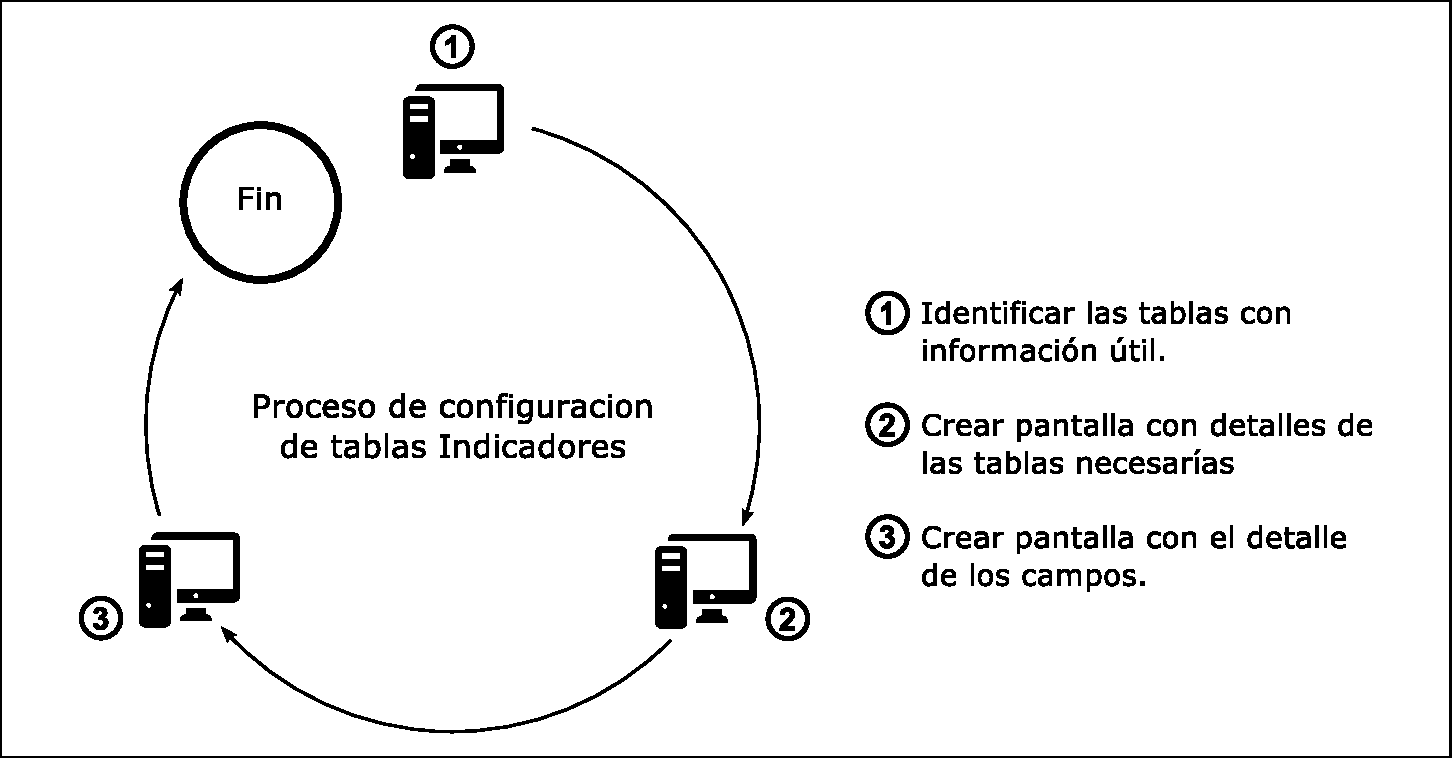
\includegraphics[width=16cm, height=8.5cm]{figuras/ConfiguracionIndicadores}
			        \caption{Diagrama del proceso de configuraci\'on de f\'ormulas de indicadores.}
			        \label{fig_ConfiguracionIndicadores}
			    \end{figure}

		    	\begin{enumerate}[1.]
		    		\item \textbf{Identificar las tablas con informaci\'on \'util.}

		    			El Sistema Integral de Indicadores necesitar\'a contar con la informaci\'on de las tablas del sistema para que \'el pueda generar consultas din\'amicas de informaci\'on, es por esto que se pide identificar las tablas que contienen informaci\'on que sea de utilidad para los fines de los indicadores.
		    			Estas tablas estar\'an disponibles para su consulta y creaci\'on de f\'ormulas permitiendo al usuario la facilidad de consultar cualquier campo que le sea de utilidad.
		    		\item \textbf{Crear pantalla con detalles de las tablas necesarias.}

		    			Este punto consta de realizar el dise\~no de una pantalla  que permita mostrar las tablas en una pantalla para poder ser consultadas y aplicadas directamente a las formulas del sistema.
						Los datos a mostrar en la pantalla son solamente el nombre de la tabla, permitiendo con esto navegar y ubicar los datos de mejor manera. La pantalla de tablas por solicitud del usuario mostrara todas las tablas de la base de datos.
						Estas tablas se mostraran en una lista en el m\'odulo de creaci\'on de f\'ormulas.
					\item \textbf{Crear pantalla con el detalle de los campos.}

						Esta pantalla ser\'a para complementar la pantalla tablas ya que el detalle de los campos de de cada tabla se mostrara en una segunda lista en el m\'odulo de creaci\'on de f\'ormulas, permitiendo con esto tener a la mano todos las herramientas necesarias para el dise\~no de estas.

		    	\end{enumerate}

		    \subsubsection{Proceso de datos}

		    	En este proceso se realizar\'a una de las tareas m\'as delicadas del sistema, ya que es aqu\'i donde se procesar\'a la informaci\'on de los indicadores.\\

				En este proceso se realizaran los c\'alculos de los indicadores, realizando el registro de los datos para tener la informaci\'on organizada seg\'un los datos reales y adem\'as para hacer m\'as eficiente la consulta de informaci\'on.\\

				En este paso se realizarla lo descrito  en la figura \ref{fig_ProcesoIndicador}

				\begin{figure}[H]
			        \centering
			        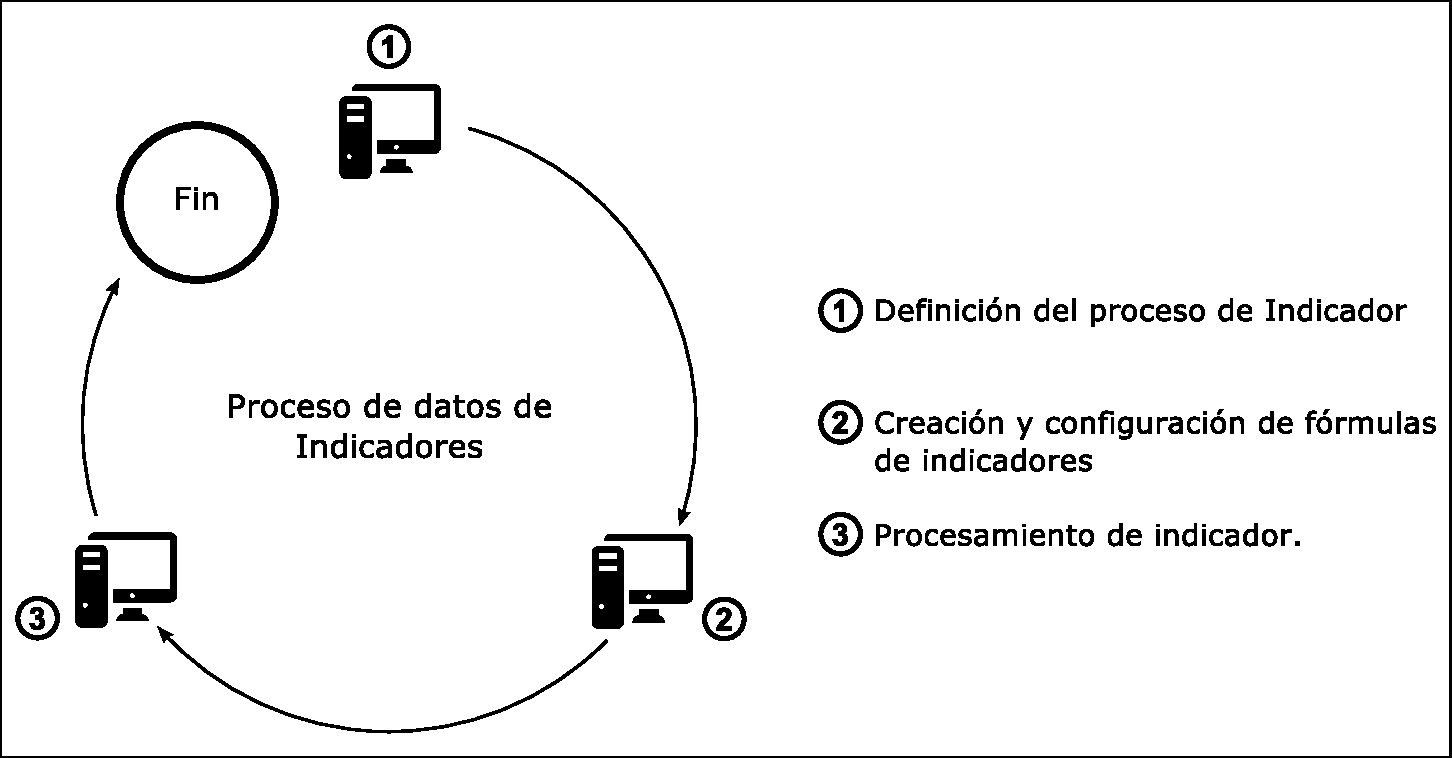
\includegraphics[width=16cm, height=8.5cm]{figuras/ProcesoIndicadores}
			        \caption{Diagrama del proceso de informaci\'on de indicadores.}
			        \label{fig_ProcesoIndicador}
			    \end{figure}

			    La definici\'on de los indicadores es la parte en donde se definen los datos para generar los resultados de los indicadores, el cual se realizara de acuerdo a los lineamientos del Instituto Tecnol\'ogico de Tl\'ahuac el cual establece que la informaci\'on se organizar\'a primeramente por instituci\'on, despu\'es se especificar\'a el departamento al que pertenece el indicador y por \'ultimo se organizar\'an por un rango de fechas especificado manualmente. Este rango de fechas podr\'a ser utilizado en la programaci\'on de las formulas permitiendo filtrar los datos.

			    \begin{enumerate}[1.]
		    		\item \textbf{Definic\'ion del proceso de indicador.}

		    			Este proceso consta de realizar la creaci\'on del proceso de indicador que se desee, para el cual se necesitan los siguientes datos:
		    			\begin{itemize}
		    				\item \textbf{ID instituci\'on:} Este campo contendr\'a el ID de la instituci\'on a la que pertenece el indicador, este campo formar\'a parte de la llave para identificar el indicador.
		    				\item \textbf{Departamento:} Este campo es el n\'umero de departamento.
		    				\item \textbf{N\'umero interno del proceso:} Este campo se autogenerara cuando se crea un nuevo proceso, ya que es \'unico para poder identificar los procesos dentro de todo el sistema.
		    				\item \textbf{Descripci\'on:} Este campo contendr\'a el detalle del contenido del indicador, permitiendo tener un resumen r\'apido del mismo.
		    				\item \textbf{Colecci\'on de f\'ormulas:} Este campo contendr\'a el n\'umero de colecci\'on que se utilizara para realizar el c\'alculo del indicador.
		    				\item \textbf{Fecha inicial:} Fecha de inicio del proceso.
		    				\item \textbf{Fecha final:} Fecha de fin del proceso.
		    				\item \textbf{Responsable:} Este campo es para almacenar el puesto o el nombre del responsable de calcular la informaci\'on de este indicador.
		    				\item \textbf{Unidad de medida:} Especifica la unidad que se utiliza para medir el indicador, este regularmente es un porcentaje.
		    			\end{itemize}

		    		\item \textbf{Configuraci\'on de f\'ormulas de indicadores.}

		    			Este proceso consiste en realizar la configuraci\'on de las f\'ormulas que permitir\'an de manera din\'amica obtener los datos configurados en la misma.

						Para realizar la configuraci\'on de la misma es necesario conocer algunos de los elementos que se pueden utilizar en las mismas los cuales son:
						\begin{itemize}
							\item F\'ormulas definidas en el sistema
							\item F\'ormulas de  Microsoft Excel
						\end{itemize}

						\textbf{F\'ormulas definidas en el sistema:} Esta funcionalidad permite realizar acciones generales basadas en funciones parametrizables, las cuales se podr\'an acceder con la siguiente nomenclatura NOMBRE\_FUNCION (PARAMETRO\_1, PARAMETRO\_2 ... PARAMETRO\_N).

						Con esto la primera capa de resoluci\'on de f\'ormulas nos permite obtener datos procesados en f\'ormulas que se pueden programar en c\'odigo, ampliando la potencia de la resoluci\'on delas mismas.

						\textbf{F\'ormulas de Microsoft Excel:} Esta funcionalidad es el segundo y \'ultimo de los niveles de resoluci\'on de f\'ormulas del sistema de indicadores, ya que al tener los datos obtenidos mediante la resoluci\'on de f\'ormulas de sistema, podemos realizar la resoluci\'on de f\'ormulas de Excel, permitiendo usar la potencia del motor de f\'ormulas de dicho software, y al tener esta posibilidad se pueden obtener los resultados como si estuvi\'eramos en el mismo software.

					\item \textbf{Procesamiento del indicador.}

						Este es el paso final del proceso de datos el cual consiste en realizar el procesamiento de las f\'ormulas y almacenamiento de dichos datos.

						Este proceso se plane\'o con el fin de tener informaci\'on espec\'ifica adem\'as de registrar estos datos en la base de datos para mejorar la eficiencia de la visualizaci\'on de los indicadores. Si este paso no existiera, la resoluci\'on de las f\'ormulas se tendr\'ia que realizar cada que un indicador se visualice generando con esto posibles inconsistencias en la informaci\'on por la adici\'on  nuevos datos, adem\'as de lentitud al momento de usar el sistema.

		    	\end{enumerate}

	\section{Dise\~no del sistema}
		Para el dise\~no del sistema se tomar\'an dos puntos de la metodolog\'ia de cascada los cuales son:
		\begin{itemize}
			\item Estructura de los datos.
			\item Caracterizaci\'on de la interfaz.
		\end{itemize}

		\subsection{Estructura de los datos}

			Para la creaci\'on de la base de datos del Sistema Integral de Indicadores es necesario identificar las entidades principales para poder comenzar con el proceso de dise\~no de la misma. Las entidades que se utilizar\'an en el sistema son:
			\begin{itemize}
				\item Departamentos.
				\item F\'ormulas.
				\item Grupos de f\'ormulas.
				\item Proceso.
			\end{itemize}

			Estas entidades est\'an ligadas con una que ya existe llamada Instituci\'on, la cual tiene la informaci\'on de las instituciones que administra el sistema.\\

			Para relacionar las entidades identificadas se cre\'o un diagrama entidad-relaci\'on como se muestra en la figura \ref{fig_DEntidadRel}.

			\begin{figure}[H]
		        \centering
		        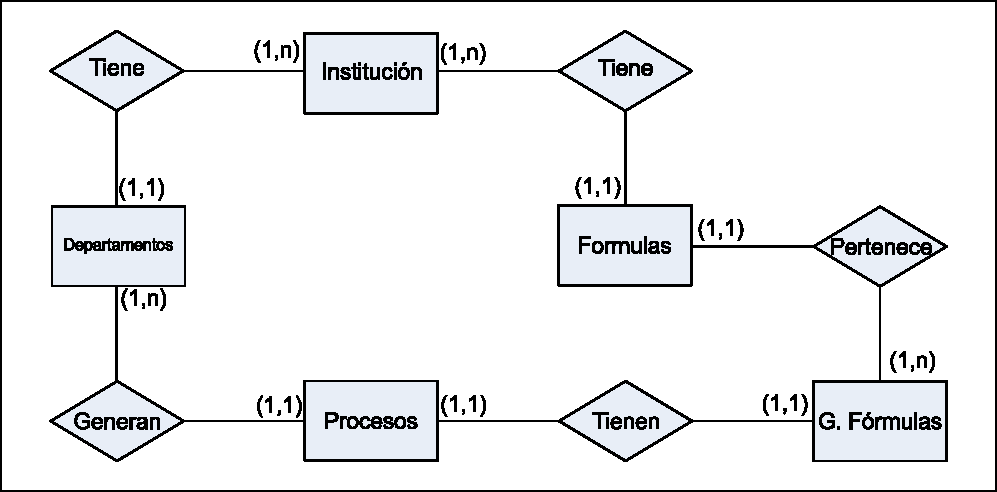
\includegraphics[width=16cm, height=8.5cm]{figuras/DEntidadRel}
		        \caption{Diagrama entidad relaci\'on del sistema de indicadores.}
		        \label{fig_DEntidadRel}
		    \end{figure}

		    \begin{itemize}
		    	\item \textbf{instituci\'on:} Esta entidad es parte del sistema general del Tecnol\'ogico de Tl\'ahuac por lo que solamente haremos referencia a ella para validar la integridad de los datos verificando que los indicadores est\'en ligados a una instituci\'on existente.
		    	\item \textbf{Departamentos:} La entidad departamentos contendr\'a la informaci\'on necesaria de cada departamento como son un identificador, su nombre y descripci\'on. Posteriormente se podr\'an agregar campos para futuras funcionalidades.
		    	\item \textbf{Formulas:} Esta entidad contendr\'a la informaci\'on de las formulas necesaria para ser identificada en el proceso. La informaci\'on que se requiere es la instituci\'on, identificador, nombre y la definici\'on de la f\'ormula. Posteriormente se pueden a\~nadir campos para futuras funcionalidades.
		    	\item \textbf{GFormulas:} Esta entidad est\'a encargada de agrupar las formulas en grupos. Estos grupos ser\'an utilizados para ser procesados en un proceso de indicadores, esta entidad se considerar\'a una entidad compuesta partiendo los datos en encabezado y detalle, permitiendo con esto evitar la redundancia de datos.
		    	\item \textbf{Procesos:} Esta entidad es la parte m\'as importante del sistema de indicadores, pues es en ella donde se almacena el resultado del c\'alculo y avance de los procesos de indicadores. Esta es considerada una entidad compuesta partiendo los datos en encabezado y detalle.
		    \end{itemize}

		    Despu\'es de identificar las entidades compuestas el diagrama sufre algunos cambios, los cuales se muestran en la figura \ref{fig_DEntidadRelComp}.

		    \begin{figure}[H]
		        \centering
		        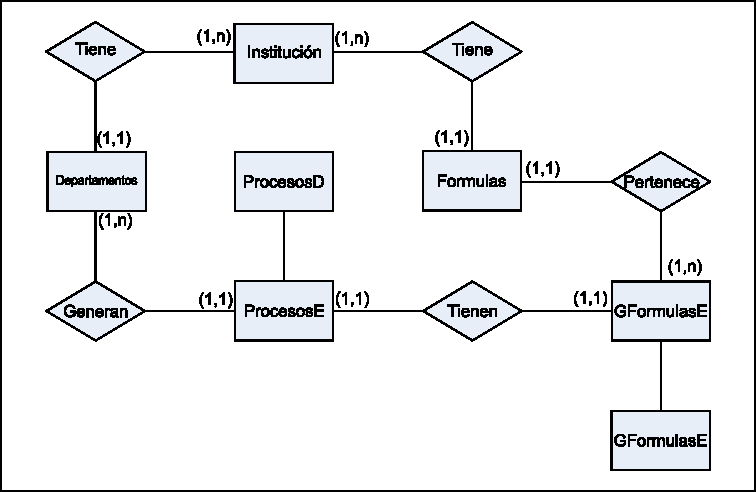
\includegraphics[width=16cm, height=8.5cm]{figuras/DEntidadRelComp}
		        \caption{Diagrama entidad relaci\'on con tablas compuestas del sistema de indicadores.}
		        \label{fig_DEntidadRelComp}
		    \end{figure}

		    \subsubsection{Definici\'on del diccionario de datos del sistema}

		    	De acuerdo a la definici\'on de los datos, se puede generar el diagrama relacional indicando como es que los datos estarán organizados en la base de datos. La figura \ref{fig_DEntidadRelComp} ilustra este diagrama.

		    	\begin{figure}[H]
			        \centering
			        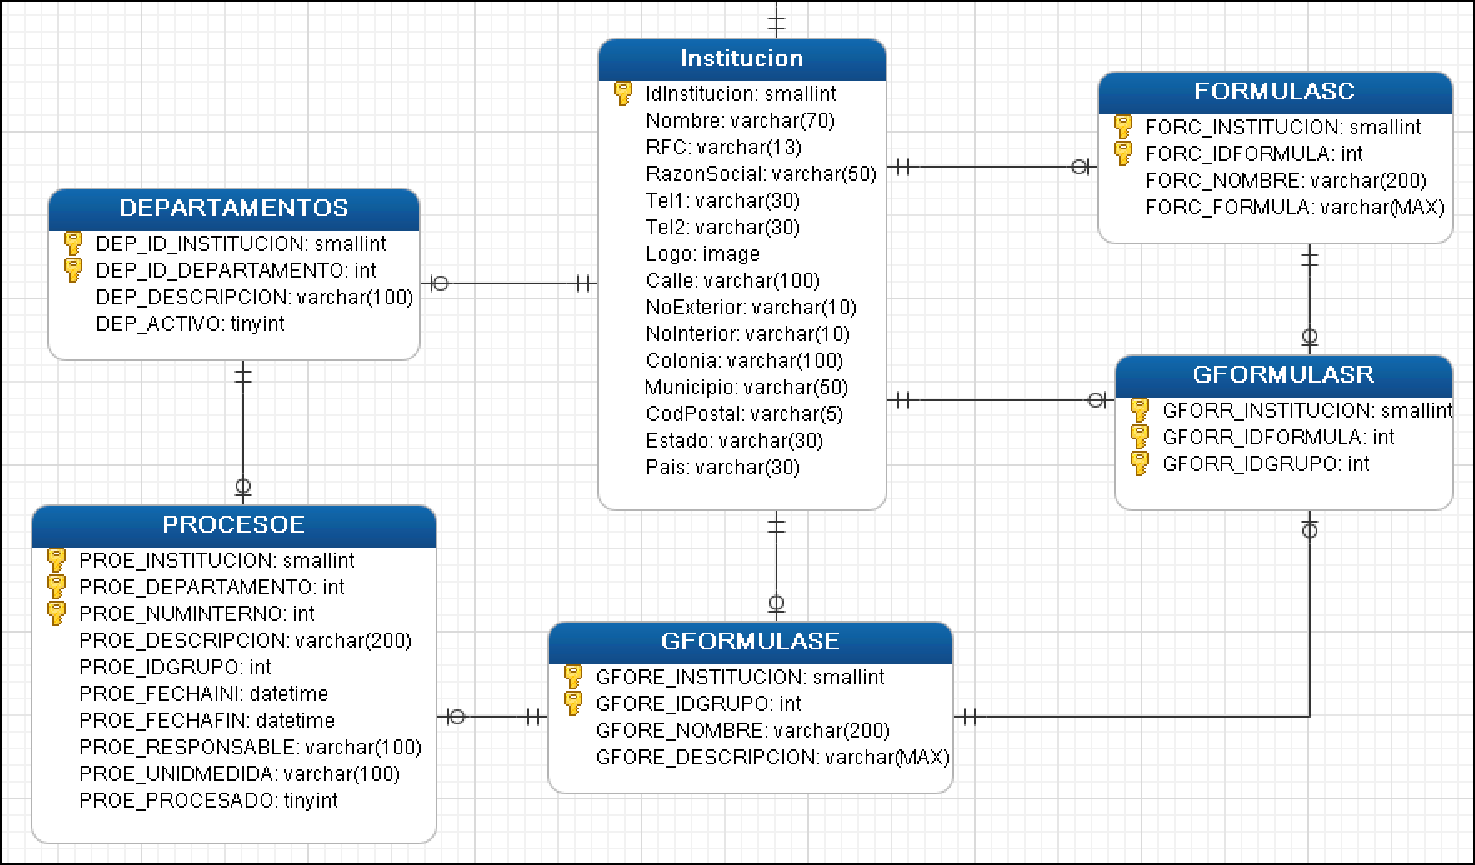
\includegraphics[width=16cm, height=8.5cm]{figuras/Relacional}
			        \caption{Diagrama relaional con campos del sistema de indicadores.}
			        \label{fig_DEntidadRelComp}
			    \end{figure}

		    \subsubsection{Definici\'on del diccionario de datos del sistema}

		    	De acruerdo a los diagramas anteriores, se procede a realizar la definicion del diccionario de datos para la

		    	\begin{table}[H]
				\centering
				\caption{Detalle de los campos de la tabla departamentos.}
				\label{tab_departamentos}
					\begin{tabular}{|l|c|c|c|c|c|c|}
						\hline
						\rowcolor[HTML]{329A9D} 
						\multicolumn{7}{|c|}{\cellcolor[HTML]{329A9D}DEPARTAMENTOS}                                                      \\ \hline
						\rowcolor[HTML]{00D2CB} 
						\multicolumn{1}{|c|}{\cellcolor[HTML]{00D2CB}Nombre} & Tipo     & TipoNativo & Longitud & Precisi\'on & Orden & PK \\ \hline
						DEP\_ACTIVO                                          & tinyint  & tinyint    & 1        & 3         & 4     & No \\ \hline
						DEP\_ID\_INSTITUCION                                 & smallint & smallint   & 2        & 5         & 1     & Si \\ \hline
						DEP\_ID\_DEPARTAMENTO                                & int      & int        & 4        & 10        & 2     & Si \\ \hline
					\end{tabular}
				\end{table}


				\begin{table}[H]
					\centering
					\caption{Detalle de los campos de la tabla formulasc.}
					\label{tab_formulasc}
					\begin{tabular}{|l|c|c|c|c|c|c|}
						\hline
						\rowcolor[HTML]{329A9D} 
						\multicolumn{7}{|c|}{\cellcolor[HTML]{329A9D}FORMULASC}                                                          \\ \hline
						\rowcolor[HTML]{00D2CB} 
						\multicolumn{1}{|c|}{\cellcolor[HTML]{00D2CB}Nombre} & Tipo     & TipoNativo & Longitud & Precisi\'on & Orden & PK \\ \hline
						FORC\_INSTITUCION                                    & smallint & smallint   & 2        & 5         & 1     & Si \\ \hline
						FORC\_IDFORMULA                                      & int      & int        & 4        & 10        & 2     & Si \\ \hline
						FORC\_NOMBRE                                         & varchar  & varchar    & 200      & 200       & 3     & No \\ \hline
						FORC\_FORMULA                                        & varchar  & varchar    & Max      & Max       & 4     & No \\ \hline
					\end{tabular}
				\end{table}

				\begin{table}[H]
					\centering
					\caption{Detalle de los campos de la tabla gformulase.}
					\label{tab_gformulase}
					\begin{tabular}{|l|l|l|l|l|l|l|}
						\hline
						\rowcolor[HTML]{329A9D} 
						\multicolumn{7}{|c|}{\cellcolor[HTML]{329A9D}GFORMULASE}                       \\ \hline
						\rowcolor[HTML]{00D2CB} 
						Nombre             & Tipo     & TipoNativo & Longitud & Precisi\'on & Orden & PK \\ \hline
						GFORE\_INSTITUCION & smallint & smallint   & 2        & 5         & 1     & Si \\ \hline
						GFORE\_IDGRUPO     & int      & int        & 4        & 10        & 2     & Si \\ \hline
						GFORE\_NOMBRE      & varchar  & varchar    & 200      & 200       & 3     & No \\ \hline
						GFORE\_DESCRIPCION & varchar  & varchar    & Max      & Max       & 4     & No \\ \hline
					\end{tabular}
				\end{table}

				\begin{table}[H]
					\centering
					\caption{Detalle de los campos de la tabla gformulasr.}
					\label{tab_gformulasr}
					\begin{tabular}{|c|c|c|c|c|c|c|}
						\hline
						\rowcolor[HTML]{329A9D} 
						\multicolumn{7}{|c|}{\cellcolor[HTML]{329A9D}GFORMULASR}                       \\ \hline
						\rowcolor[HTML]{00D2CB} 
						Nombre             & Tipo     & TipoNativo & Longitud & Precisi\'on & Orden & PK \\ \hline
						GFORR\_INSTITUCION & smallint & smallint   & 2        & 5         & 1     & Si \\ \hline
						GFORR\_IDFORMULA   & int      & int        & 4        & 10        & 2     & Si \\ \hline
						GFORR\_IDGRUPO     & int      & int        & 4        & 10        & 3     & Si \\ \hline
					\end{tabular}
				\end{table}

				\begin{table}[H]
					\centering
					\caption{Detalle de los campos de la tabla procesoe.}
					\label{tab_procesoe}
					\begin{tabular}{|l|c|c|c|c|c|c|}
						\hline
						\rowcolor[HTML]{329A9D} 
						\multicolumn{7}{|c|}{\cellcolor[HTML]{329A9D}PROCESOE}                                                           \\ \hline
						\rowcolor[HTML]{00D2CB} 
						\multicolumn{1}{|c|}{\cellcolor[HTML]{00D2CB}Nombre} & Tipo     & TipoNativo & Longitud & Precisi\'on & Orden & PK \\ \hline
						PROE\_PROCESADO                                      & tinyint  & tinyint    & 1        & 3         & 10    & No \\ \hline
						PROE\_INSTITUCION                                    & smallint & smallint   & 2        & 5         & 1     & Si \\ \hline
						PROE\_DEPARTAMENTO                                   & int      & int        & 4        & 10        & 2     & Si \\ \hline
						PROE\_NUMINTERNO                                     & int      & int        & 4        & 10        & 3     & Si \\ \hline
						PROE\_IDGRUPO                                        & int      & int        & 4        & 10        & 5     & No \\ \hline
						PROE\_FECHAINI                                       & datetime & datetime   & 8        & 23        & 6     & No \\ \hline
						PROE\_FECHAFIN                                       & datetime & datetime   & 8        & 23        & 7     & No \\ \hline
						PROE\_DESCRIPCION                                    & varchar  & varchar    & 200      & 200       & 4     & No \\ \hline
						PROE\_RESPONSABLE                                    & varchar  & varchar    & 100      & 100       & 8     & No \\ \hline
						PROE\_UNIDMEDIDA                                     & varchar  & varchar    & 100      & 100       & 9     & No \\ \hline
					\end{tabular}
				\end{table}

				\begin{table}[H]
					\centering
					\caption{Detalle de los campos de la tabla procesod.}
					\label{tab_procesod}
					\begin{tabular}{|l|c|c|c|c|c|c|}
						\hline
						\rowcolor[HTML]{329A9D} 
						\multicolumn{7}{|c|}{\cellcolor[HTML]{329A9D}PROCESOD}                                                             \\ \hline
						\rowcolor[HTML]{00D2CB} 
						\multicolumn{1}{|c|}{\cellcolor[HTML]{00D2CB}Nombre} & Tipo     & TipoNativo & Longitud & Precisi\'on & Orden & PK \\ \hline
						PROD\_INSTITUCION                                    & smallint & smallint   & 2        & 5           & 1     & Si \\ \hline
						PROD\_NUMINTERNO                                     & int      & int        & 4        & 10          & 2     & Si \\ \hline
						PROD\_CONSECUTIVO                                    & int      & int        & 4        & 10          & 3     & Si \\ \hline
						PROD\_FORMULASIS                                     & varchar  & varchar    & Max      & Max         & 4     & No \\ \hline
						PROD\_FORMULAPRE                                     & varchar  & varchar    & Max      & Max         & 5     & No \\ \hline
						PROD\_FORMULARES                                     & varchar  & varchar    & Max      & Max         & 6     & No \\ \hline
					\end{tabular}
				\end{table}

				Con esto la definici\'on de los datos queda completa, permitiendo tener los argumentos suficientes para la descripci\'on de las interfaces.





	\section{Caracterizaci\'on de la interfaz}

		Para la definici\'on de la funcionalidad de la interfaz se tomaran en cuenta los siguientes requerimientos generales:
		\begin{itemize}
			\item Los tipos de dato de los componentes de entrada de las interfaces estar\'an definidos de acuerdo al tipo de dato nativo en la BD, esto para mejorar la experiencia del usuario.
			\item Todas las entradas de datos se mostrar\'an en ventanas emergentes.
			\item La visualizaci\'on de los datos se har\'a en una tabla para mejorar la accesibilidad de los datos
			\item Las acciones propias a los registros serán colocadas a la derecha de la tabla, estas no tendr\'an t\'itulo de encabezado.
			\item Se crearan los botones de navegaci\'on del sistema en la parte superior derecha de las tablas, estas acciones ser\'an determinadas por m\'odulo.
			\item En el caso de que no existan registros para mostrar en el m\'odulo, deber\'a de mostrar un mensaje descriptivo a la situaci\'on, dejando invisibles los encabezados de la tabla propia del m\'odulo.
		\end{itemize}

		En el caso de algunos m\'odulos, se deber\'an de tomar algunas consideraciones especiales las cuales se describe continuaci\'on:

		\begin{itemize}
			\item \textbf{Colecciones:} En el caso de este formulario se deber\'a agregar una columna que muestre un bot\'on, este bot\'on re direccionara al formulario DetalleColecciones.
			\item \textbf{DetalleColecciones:} Este formulario contara \'unicamente con las funciones de agregar y eliminar, se deshabilita la funci\'on de actualizar ya que aqu\'i no se pueden modificar las formulas si no solo agregarlas o eliminarlas. 

			La funcionalidad de agregar se mostrara en una ventana emergente la cual tendr\'a \'unicamente una lista multi-selecci\'on que mostrara las f\'ormulas que est\'an disponibles para ser agregadas a la colecci\'on.
			\item \textbf{Proceso:} Este dormulario mostrara los registros del encabezado de los procesos con las siguientes funcionalidades.
			\begin{itemize}
				\item \textbf{Crear:} Esta funcionalidad permitir\'a crear un nuevo proceso.
				\item \textbf{Actualizar:} Esta funcionalidad permite actualizar los datos del periodo. Cuando se realiza esta acci\'on es importante mencionar que el periodo puede que necesite reprocesarse, ya que los datos como las fechas de inicio y fin o el n\'umero de colecci\'on de f\'ormulas afectan directamente en el resultado.
				\item \textbf{Eliminar:} Esta funcionalidad permite eliminar un proceso. Es importante destacar que al eliminar un proceso se eliminaran tanto los registros en el encabezado y el detalle.
				\item \textbf{Procesar:} Esta funcionalidad ejecuta la resoluci\'on de f\'ormulas del sistema guardando los resultados en el detalle del proceso.
				\item \textbf{Detalle:} Esta funcionalidad muestra los registros que se encuentran en el detalle del proceso. Este formulario es solo de consulta por lo que no se tendr\'a ninguna funcionalidad.
			\end{itemize}
		\end{itemize}



	\chapter{Pruebas y resultados}

En este cap�tulo se presentan algunos de los aspectos m�s relevantes para desarrollar la escritura de los resultados de aprendizaje asociados a una determinada  materia o asignatura. Se trata de definir qu� se entiende por resultados de aprendizaje, el desarrollo de herramientas para su redacci�n y algunas claves y recomendaciones, para valorar su calidad una vez escritos con el fin de poder revisarlos con profundidad.\\

Asimismo, tambi�n se desarrolla ampliamente una serie de recomendaciones para el desarrollo de pruebas  que sean eficaces en cuanto a su relaci�n con los resultados de aprendizaje fundamentalmente, pero tambi�n respecto a las modalidades y m�todos de ense�anza utilizados.\\


\section{Gu�a de vocabulario para la escritura del componente verbal de aprendizaje}

Encontrar las palabras adecuadas en la escritura de un resultado este puede resultar una tarea dif�cil, especialmente si tenemos presentes otros elementos del dise�o de un cap�tulo: competencias, intenciones u objetivos del asesor.\\
 
\subsection{Actividades que proporcionan evidencia de conocimiento}

Definir, describir, identificar, etiquetar, listar, nombrar, reproducir, declarar, recordar, seleccionar, declarar, se consciente de, extraer, organizar, escribir, reconocer, medir,  subrayar, repetir, relacionar, conocer, asociar.

\subsection{Actividades que proporcionan evidencia de comprensi�n}
 
Interpretar, traducir, estimar, justificar, comprender, convertir, clarificar, defender, distinguir, explicar, extender, generalizar, ejemplificar, dar ejemplos de, inferir, parafrasear, predecir, rescribir, resumir, discutir, ejecutar, reportar, presentar, identificar, ilustrar, indicar, encontrar, seleccionar, comprender, representar, formular, juzgar, contrastar, clasificar, expresar, comparar.

\subsection{Actividades que proporcionan evidencia de aplicaci�n} 

Aplicar, resolver, construir, demostrar, cambiar, calcular, descubrir, manipular, modificar, operar, predecir, preparar, producir, relacionar, mostrar, usar, dar ejemplos, ejemplificar, dibujar, seleccionar, explicar c�mo, encontrar, elegir, evaluar, practicar, operar, ilustrar, verificar.

\subsection{Actividades que proporcionan evidencia de an�lisis}
 
Reconocer, distinguir entre, evaluar, analizar, diferenciar, identificar, ilustrar c�mo, inferir, destacar, se�alar, relacionar, seleccionar, separar, dividir, subdividir, comparar, contrastar, justificar, resolver, examinar, concluir, criticar, cuestionar, diagnosticar, identificar, categorizar, elucidar.

\subsection{Actividades que proporcionan evidencia de s�ntesis}
 
Proponer, presentar, estructurar, integrar, formular, ense�ar, desarrollar, combinar, compilar, componer, crear, dise�ar, explicar, generar, modificar, organizar, planificar, reestructurar, reconstruir, relacionar, reorganizar, revisar, escribir, resumir, conectar, reportar, alterar, argumentar, ordenar, seleccionar, gestionar, generalizar, precisar, derivar, concluir, construir, engendrar, sintetizar, agrupar, sugerir, extender.

\subsection{Actividades que proporcionan evidencia de evaluaci�n}
 
Juzgar, evaluar, concluir, comparar, contrastar, describir c�mo, criticar, discriminar, justificar, defender, evaluar, valorar, determinar, elegir, cuestionar, puntuar.\\

Analizando los componentes del �ltimo ejemplo:\\

			\begin{center}
			Verbo + Contenido + Naturaleza
			\end{center}


\section{Consejos para la escritura de pruebas y resultados}

\begin{itemize}
	\item En cualquier tipo de prueba y resultado se necesita que exista alguna clase de declaraci�n, bien sobre lo que el estudiante har� 					bien una referencia de la calidad del trabajo que ser� clave en la tarea para alcanzar los criterios de �xito marcados en �ste.
	\item Las pruebas y resultados deben evaluar o relacionarse con el aprendizaje que se menciona en el resultado.
	\item Redactar un punto cr�tico, o umbral, en los resultados proporciona m�s detalle a la evaluaci�n y permite precisar que el aprendizaje se ha conseguido.
\end{itemize}




\section{Ejemplos de redacci�n de criterios de evaluaci�n}
Resultado de aprendizaje: Al finalizar este cap�tulo, se espera que el estudiante sea capaz de explicar y demostrar los principales resultados de un reporte de residencias profesionales. Algunos criterio para las pruebas y resultados son:\\

\begin{itemize}
	\item Las pruebas y resultados deben estar escritas en procesador de textos y debe tener una extensi�n de superior a 5 cuartillas sobre 				el tema proporcionado.
	\item El resultado debe relacionarse con su prueba, as� como con el t�tulo del proyecto, debe estar claramente escrito y estructurado, 					demostrar la contribuci�n de lecturas complementarias y reflexi�n propia.
	\item El estudiante debe ser capaz de explicar c�mo  los resultados de las pruebas demuestran estos rasgos y c�mo contribuyen a su 							efectividad global.
	\item El alumno demostrar� al menos tres ejemplos de refuerzo positivo para mejorar las conductas.
\end{itemize}
   

	\chapter{Conclusiones}

\section{Conclusiones finales}
	Al principio de las conclusiones se debe volver a repetir lo que se hizo en el trabajo. Se
	repite cu�l era el objetivo y se describe en pocas palabras, muy concisas y concretas, el tra-
	bajo realizado. Luego de describir lo que se hizo, se destacan los aspectos m�s importantes
	de este trabajo y se concluye algo sobre ellos. Por ejemplo, se pueden destacar los puntos
	m�s dif�ciles o los que significaron un reto importante, o lo que present� mayores dificultades
	para resolverse. Si hubo un cambio de rumbo en cuanto a los objetivos planteados originalmente, 
	tambi�n se puede explicar aqu�. Si se analizaron varias alternativas de soluci�n de
	un problema, estas alternativas se pueden explicar en esta secci�n y al final se dice c�mo se
	tom� la decisi�n de elegir una soluci�n y cu�l fue esta soluci�n.\\
	
	Evite redactar las conclusiones como una lista de �temes, se pueden hacer as� para la
	presentaci�n, pero no en la escritura del informe. Las conclusiones deben seguir una redacci�n
	fluida. Al final de las conclusiones se pueden incluir algunas recomendaciones espec�ficas que el
	autor del trabajo cree que puedan ser �tiles, pero que ya no le compete llevarlas a cabo. 
	
	
	
\begin{enumerate}
	\item Formato b�sico para las conclusiones
		\begin{itemize}
			\item \textbf{B�squeda}: �Qu� se hizo para reunir informaci�n sobre el problema?
			\item \textbf{Hip�tesis}: �Qu� es lo que se est� comprobando con el experimento?
			\item \textbf{Motivo de tu hip�tesis}: �C�mo  ha ocurrido la hip�tesis?
			\item \textbf{Procedimiento}: Explica lo que est�s haciendo.
			\item \textbf{An�lisis/Resultados}: �Qu� ha pasado? Se proporcionan los datos aqu�.
			\item \textbf{Conclusi�n}: �Cu�l es tu conclusi�n sobre el reporte? �Por qu�?
		\end{itemize}
		
	\item Toma notas. Es importante para usarlas despu�s
	\begin{itemize}
		\item Trata de ser conciso: no escribir cosas superfluas que no se  necesiten.
		\item Puede ser tentador escribir m�s cosas de las que se deben, pero si ya est� la informaci�n importante, no escribas nada m�s.
	\end{itemize}
	
	\item Aprende la hip�tesis. Cada experimento cient�fico tiene una. La hip�tesis es una afirmaci�n que se espera que ocurra al hacer el 		experimento. El resultado es aprobar o descartar tu hip�tesis.
	
	\item Comprende si la hip�tesis ha sido confirmada o descartada. Escribe eso claramente en el informe.
	
	\item Analiza los datos presentados correctamente. Preg�ntate por qu� ha salido ese resultado. Si tienes una respuesta, apuntala en tus notas para que no se te olvide. Abajo vienen los tipos de datos para los experimentos de laboratorio:
	\begin{itemize}
		\item Datos basados en valores: todos tus datos est�n en forma de n�mero. En este caso deber�s dibujar un gr�fico para presentar tu 						conclusi�n. Haz relaciones entre los factores probados en el experimento.
		\item Datos basados en hechos. Tus datos se basan en observaciones, como cambios de color, tipos de reacci�n y otros fen�menos que no 					incluyan n�meros.
	\end{itemize}
	\item Identifica una fuente de error experimental (opcional). Si algo ha pasado que haya alterado el resultado y no deber�a haber 							ocurrido, expl�calo. Por ejemplo, el viento ha reducido la temperatura de los reactores y por ello la reacci�n ha ocurrido m�s 						despacio de lo que deber�a.
	
	\item Termina con una conclusi�n. Escribe de manera ordenada lo que hayas aprendido en el experimento. �La hip�tesis te ha ense�ado 						algo? �Los resultados eran los que esperabas?
\end{enumerate}





	\input{Referencias/referencias}	
	\appendix
	\chapter{Lineamientos generales}



De acuerdo a la Real Academia Espa\~nola (REA) se llama sigla tanto a la palabra formada por las iniciales de los t\'erminos que integran una denominaci\'on compleja, como a cada una de esas letras iniciales. Las siglas se utilizan para referirse de forma abreviada a organismos, instituciones, empresas, objetos, sistemas, asociaciones, etc.



\begin{enumerate}[1)] 

	\item \textbf{Tipos de siglas seg\'un su lectura}
		\begin{enumerate}[a)]
			\item {Hay siglas que se leen tal como se escriben, las cuales reciben tambi\'en el nombre de acr\'onimos: ONU, OTAN, ovni. Muchas de estas siglas acaban incorpor\'andose como sustantivos al l\'exico com\'un. Cuando una sigla est\'a compuesta solo por vocales, cada una de ellas se pronuncia de manera independiente y conserva su acento fon\'etico: OEA (\textit{Organizaci\'on de Estados Americanos}) se pronuncia [\'o-\'e-\'a].}

			\item {Hay siglas cuya forma impronunciable obliga a leerlas con deletreo: \textit{FBI} [\'efe-b\'e-\'i], \textit{DDT} [d\'e-d\'e-t\'e]. Integrando las vocales necesarias para su pronunciaci\'on, se crean a veces, a partir de estas siglas, nuevas palabras: \textit{elep\'e} (de \textit{LP}, sigla del ingl. \textit{long play} 'larga duraci\'on').}
			
			\item {Hay siglas que se leen combinando ambos m\'etodos: \textit{CD-ROM} [se-de-rr\'on, ze-de-rr\'en] (sigla del ingl. \textit{Compact Disc Read-Only Memory} 'disco compacto de solo lectura'). Tambi\'en en este caso pueden generarse palabras a partir de la sigla: \textit{cederr\'on}.}
			
	\end{enumerate}

	\item \textbf{Plural}. Aunque en la lengua oral tienden a tomar marca de plural ([oenej\'es] = 'organizaciones no gubernamentales'), son invariables en la escritura: las \textit{ONG}; por ello, cuando se quiere aludir a varios referentes es recomendable introducir la sigla con determinantes que indiquen pluralidad: \textit{Representantes de algunas/varias/numerosas ONG se reunieron en Madrid}. Debe evitarse el uso, copiado del ingl\'es, de realizar el plural de las siglas a\~nadiendo al final una \textit{s} min\'uscula, precedida o no de ap\'ostrofo: {\color{red} CD's, ONG's}.

	\item \textbf{G\'enero}. Las siglas adoptan el g\'enero de la palabra que constituye el n\'ucleo de la expresi\'on abreviada, que normalmente ocupa el primer lugar en la denominaci\'on: el FMI, por el \textit{Fondo Monetario Internacional}; la OEA, por la \textit{Organizaci\'on de Estados Americanos}; la UNESCO, por la \textit{United Nations Educational, Scientific and Cultural Organization} ('Organizaci\'on de Naciones Unidas para la Educaci\'on, la Ciencia y la Cultura'). Las siglas son una excepci\'on a la regla que obliga a utilizar la forma \textit{el} del art\'iculo cuando la palabra femenina que sigue comienza por /a/ t\'onica.

	\item \textbf{Ortograf\'ia}
		\begin{enumerate}[a)]
		\item {Las siglas se escriben hoy sin puntos ni espacios blancos de separaci\'on. S\'olo se escribe punto tras las letras que componen las siglas cuando van integradas en textos escritos enteramente en may\'usculas.}

		\item {Las siglas presentan normalmente en may\'uscula todas las letras que las componen (\textit{OCDE, DNI, ISO}) y, en ese caso, no llevan nunca tilde; as\'i, \textit{CIA} (del ingl. \textit{Central Intelligence Agency}) se escribe sin tilde, a pesar de pronunciarse [s\'ia, z\'ia], con un hiato que exigir\'ia acentuar gr\'aficamente la i. Las siglas que se pronuncian como se escriben, esto es, los acr\'onimos, se escriben solo con la inicial may\'uscula si se trata de nombres propios y tienen m\'as de cuatro letras: Unicef, Unesco; o con todas sus letras min\'usculas, si se trata de nombres comunes: uci, ovni, sida. Los acr\'onimos que se escriben con min\'usculas sí deben someterse a las reglas de acentuaci\'on gr\'afica: m\'odem.}

		\item {Si los d\'igrafos \textit{ch} y \textit{ll} forman parte de una sigla, va en may\'uscula el primer car\'acter y en min\'uscula el segundo: \textit{PCCh}, sigla de Partido Comunista de China.}

		\item {Se escriben en cursiva las siglas que corresponden a una denominaci\'on que debe aparecer en este tipo de letra cuando se escribe completa; esto ocurre, por ejemplo, con las siglas de t\'itulos de obras o de publicaciones peri\'odicas: \textit{DHLE}, sigla de Diccionario hist\'orico de la lengua espa\~nola; \textit{RFE}, sigla de Revista de Filolog\'ia Espa\~nola.}

		\item {Las siglas escritas en may\'usculas nunca deben dividirse con guion de final de l\'inea.}
	\end{enumerate}

	\item {Hispanizaci\'on de las siglas}. Siempre que sea posible, se hispanizar\'an las siglas: \textit{OTAN}, y no \textit{NATO}; \textit{ONU}, y no \textit{UNO}. Solo en casos de difusi\'on general de la sigla extranjera y dificultad para hispanizarla, o cuando se trate de nombres comerciales, se mantendr\'a la forma original: \textit{Unesco}, sigla de \textit{United Nations Educational, Scientific and Cultural Organization}; \textit{CD-ROM}, sigla de \textit{Compact Disc Read-Only Memory}; \textit{IBM}, sigla de \textit{International Business Machines}. Tampoco deben hispanizarse las siglas de realidades que se circunscriben a un pa\'is extranjero, sin correspondencia en el propio: \textit{IRA}, sigla de \textit{Irish Republic Army}. La primera vez que se emplea una sigla en un texto, y salvo que sea de difusi\'on tan generalizada que se sepa f\'acilmente interpretable por la inmensa mayor\'ia de los lectores, es conveniente poner a continuaci\'on, y entre par\'entesis, el nombre completo al que reemplaza y, si es una sigla extranjera, su traducci\'on o equivalencia: \textit{DEA} (\textit{Drug Enforcement Administration}, departamento estadounidense de lucha contra las drogas); o bien escribir primero la traducci\'on o equivalencia, poniendo despu\'es la sigla entre par\'entesis: la Uni\'on Nacional Africana de Zimbabue (\textit{ZANU}).
	
\end{enumerate}
	
	\renewcommand\appendixname{Anexo}
	\chapter{Lineamientos para la publicaci\'on de memorias de residencias}
Documentar el c\'odigo fuente de un programa es a\~nadir suficiente informaci\'on como para explicar lo que hace, punto por punto, de forma que no s\'olo las computadoras sepan qu\'e hacer, sino que adem\'as los humanos entiendan qu\'e est\'an haciendo y por qu\'e.\\

Porque entre lo que tiene que hacer un programa y c\'omo lo hace hay una distancia impresionante: todas las horas que el programador ha dedicado a la una soluci\'on y escribirla en el lenguaje que corresponda para que la computadora la ejecute ciegamente.\\

Documentar un programa no es s\'olo un acto de buen hacer del programador, es adem\'as una necesidad que s\'olo se aprecia en su debida magnitud cuando hay errores que reparar o hay que extender el programa con nuevas capacidades o adaptarlo a un nuevo escenario. Hay dos reglas que no se deben olvidar nunca:

\begin{enumerate}[1)]
	\item 	Todos los programas tienen errores y descubrirlos s\'olo es cuesti\'on de tiempo y de que el programa tenga \'exito y se utilice frecuentemente.

	\item Todos los programas sufren modificaciones a lo largo de su vida, al menos todos aquellos que tienen \'exito
\end{enumerate}

Por una u otra raz\'on, todo programa que tenga \'exito ser\'a modificado en el futuro, bien por el programador original o por otro que le sustituya. Pensando en esta revisi\'on de c\'odigo es por lo que es importante que el programa se entienda: para poder repararlo y modificarlo.

\section{?`Qu\'{e} hay que documentar?}

Hay que a\~nadir explicaciones a todo lo que no es evidente. No hay que repetir lo que se hace, sino explicar por qu\'e se hace.
Y eso se traduce en:

\begin{itemize}
	\item ?`de qu\'e se encarga una clase? ?`un paquete?
	\item ?`qu\'e hace un m\'etodo?
	\item ?`cu\'al es el uso esperado de un m\'etodo?
	\item ?`para qu\'e se usa una variable?
	\item ?`cu\'al es el uso esperado de una variable?
	\item ?`qu\'e algoritmo estamos usando? ?`de d\'onde lo hemos sacado?
\end{itemize}

Por ejemplo, el lenguaje Java dispone de tres notaciones para introducir comentarios:\\

\begin{enumerate}[1)]
	\item \textbf{javadoc}. Comienzan con los caracteres ''/**'', se pueden prolongar a lo largo de varias l\'ineas (que probablemente comiencen con el car\'acter ''*'') y terminan con los caracteres ''*/''.
	
	\item \textbf{Una l\'inea}. Comienzan con los caracteres ''//'' y terminan con la l\'inea
	
	\item \textbf{Tipo C}. Comienzan con los caracteres ''/*'', se pueden prolongar a lo largo de varias l\'ineas (que probablemente comiencen con el car\'acter "*") y terminan con los caracteres "*/".
\end{enumerate}

Cada tipo de comentario se debe adaptar a un prop\'osito: \textbf{javadoc} es para generar documentaci\'on externa. \textbf{Una l\'inea} se usa para documentar c\'odigo que no necesite que aparezca en la documentaci\'on externa (que genere javadoc)
Este tipo de comentarios se usar\'a incluso cuando el comentario ocupe varias l\'ineas, cada una de las cuales comenzar\'a con ''//''.\textbf{Tipo C} es para eliminar c\'odigo. Ocurre a menudo que c\'odigo obsoleto no queremos que desaparezca, sino mantenerlo ''por si acaso''. Para que no se ejecute, se comenta.(En ingl\'es se suele denominar ''comment out'').\\

Es importante respetar las normas y est\'andares correspondientes a cada lenguaje de programaci\'on. As\'i como los comentarios, tambi\'en existen otras reglas que deben ser consideras al momento de insertar un c\'odigo fuente en alg\'un reporte. Algunas de estas reglas son alineaci\'on, indentado, legibilidad y otras m\'as.\\

En el siguiente c\'odigo se presenta un ejemplo del lenguaje Java, en el cual se aprecia un est\'ilo apropiado para comentar c\'odigo.

\begin{lstlisting}
import java.util.ArrayList;
import java.util.Random;
 
/**
 * Esta clase define objetos que contienen tantos enteros aleatorios entre 0 y 1000 como se le definen al crear un objeto
 * @author: Academia de Sistemas y Computacion
 * @version: 20/09/2014
**/
 
public class SerieDeAleatoriosD {
 
    //Campos de la clase
    private ArrayList<Integer> serieAleatoria;
    /**
     * Constructor para la serie de numeros aleatorios
     * @param numeroItems El parametro numeroItems define el numero de elementos que va a tener la serie aleatoria
     */
    public SerieDeAleatoriosD (int numeroItems) {
        serieAleatoria = new ArrayList<Integer> ();
        for (int i=0; i<numeroItems; i++) {  serieAleatoria.add(0);  }
        System.out.println ("Serie inicializada. El numero de elementos en la serie es: " + getNumeroItems() );
    } //Cierre del constructor
    /*
     * Metodo que devuelve el numero de items (numeros aleatorios) existentes en la serie
     * @return El numero de items (numeros aleatorios) de que consta la serie
     */
    public int getNumeroItems() { return serieAleatoria.size(); }
    /**
     * Metodo que genera la serie de numeros aleatorios
     */
    public void generarSerieDeAleatorios () {
        Random numAleatorio;
        numAleatorio = new Random ();
        for (int i=0; i < serieAleatoria.size(); i++) { serieAleatoria.set(i, numAleatorio.nextInt(1000) ); }
        System.out.print ("Serie generada! ");
    } //Cierre del metodo
} //Cierre de la clase
\end{lstlisting}

\section{Marcado de palabras clave}

Es importante que todo c\'odigo anexado sea presentable y legible, para ello se puede hacer uso de diferentes colores para diferenciar  palabras clave, clases, variables, etc. A continuaci\'on se presenta un c\'odigo en lenguaje HTML.

\begin{lstlisting}
<!DOCTYPE html>
<html>
  <head>
    <title>Canvas</title>
    <meta charset="UTF-8" />
    <style>
      #square {
        border: 1px solid black;
                transform: scale(10) rotate(3deg) translateX(0px);
                -moz-transform: scale(10) rotate(3deg) translateX(0px);
      }

            .box {              
                transition-duration: 2s;
                transition-property: transform;
                transition-timing-function: linear;
      }
    </style>
  </head>
  <body>
    <canvas id="square" width="200" height="200"></canvas>
    <script>
            var canvas = document.createElement('canvas');
            canvas.width = 200;
            canvas.height = 200;

            var image = new Image();
            image.src = 'images/card.png';
            image.width = 114;
            image.height = 158;
            image.onload = window.setInterval(function() {
                rotation();
            }, 1000/60);
   </script>
  </body>
</html>
    \end{lstlisting}

\section{Indentado}

Las normas de indentaci\'on indican la posici\'on en la que se deben colocar los diferentes elementos que se incluyen en el c\'odigo fuente, por lo que forman parte del estilo de codificaci\'on. Otro ejemplo de ello es la separaci\'on con espacios en blanco entre los diferentes elementos que componen las l\'ineas de c\'odigo.

\subsection{Objetivo de la indentaci\'on}

El objetivo fundamental de la indentaci\'on del c\'odigo fuente es facilitar su lectura y comprensi\'on. Hay dos tipos de posibles lectores del c\'odigo fuente: programas y personas. A los programas les da igual la indentaci\'on, leen bien nuestro c\'odigo siempre que cumpla la sintaxis del lenguaje. Luego la indentaci\'on debe centrarse en la lectura y comprensi\'on del c\'odigo por personas.\\

A continuaci\'on se presenta un ejemplo de identaci\'on usando el lenguaje de programaci\'on Python. Las funciones de Python no tienen begin o end expl\'icitos, ni llaves que marquen d\'onde empieza o termina su c\'odigo. El \'unico delimitador son dos puntos (:) y el indentado del propio c\'odigo.\\

\begin{lstlisting}
"""Modulo para ejemplificar el uso de *epydoc*. 
   :author: Raul Gonzalez 
   :version: 0.1"""  
  
__docformat__ = "restructuredtext"  
  
class Persona:  
    """Modela una persona."""  
    def __init__(self, nombre, edad):  
        """Inicializador de la clase `Persona`. 
           :param nombre: Nombre de la persona. 
           :param edad: Edad de la persona"""  
        self.nombre = nombre  
        self.edad = edad  
        self.mostrar_nombre()  
  
    def mostrar_nombre(self):  
        """Imprime el nombre de la persona"""  
        print "Esta es la persona %s" % self.nombre  
  
class Empleado(Persona):  
    """Subclase de `Persona` correspondiente a las personas 
       que trabajan para la organizacion. 
       :todo: Escribir implementacion."""  
    pass  
  
  
if __name__ == "__main__":  
    juan = Persona("Juan", 26) 
\end{lstlisting}
	
	\bibliographystyle{IEEEannot}
	\bibliography{biblio}
	\nocite{*}
\end{document}